\chapter{Quadratic Forms}

Symmetric matrices often see their appearance in the areas of Geometry, Statistics, Physics, and more, taking the form of \textit{quadratic forms}. They can be used to describe a family of geometric shapes known as \textit{conic sections}, including ellipses and hyperbola. A more common application of quadratic forms in Earth Sciences will be obtaining the \textit{covariance matrix} between different variables, eventually leading to \textit{Principal Component Analysis (PCA)} which breaks down the variables into isolated modes that explain the spread of their distributions. In Atmospheric Science, it is more commonly known as \textit{Empirical Orthogonal Functions (EOF)} and has been widely used to analyze prominent, large-scale climate patterns like \textit{El Niño–Southern Oscillation (ENSO)}. 

\section{Mathematical and Geometric Ideas of Quadratic Forms}
\subsection{Definition of Quadratic Forms}

The word \textit{quadratic} is commonly associated to \textit{quadratic equations} in the form of $y = ax^2 + bx + c$. \index{Quadratic Form}\keywordhl{Quadratic forms} are the generalization of quadratic equations when there are multiple variables $x_1, x_2, x_3, \ldots$: the possible quadratic forms will be made up of the usual quadratic terms $x_1^2, x_2^2, x_3^2, \ldots$, as well as the \textit{cross-product terms} $x_px_q$, $p \neq q$. The usual quadratic terms then can be seen as just another kind of cross-product terms when $p = q$. We will limit our discussion to real vector spaces.
\begin{defn}
\label{defn:quadform}
Real quadratic forms of multiple variables $\vec{x} = (x_1, x_2, x_3, \ldots)^T$ has a structure of
\begin{align*}
Q(\vec{x}) = \sum_{p=1}^{n}\sum_{q=1}^{n} \beta_{pq} x_px_q
\end{align*}
Note that it is a real scalar.
\end{defn}
For examples, in a two variables situation, $x^2 + 3xy + y^2$, $3x^2 - 4xy$ are quadratic forms, while $x^2 + y$, $xy + xy^2$ are not. Notice that $x_px_q$ and $x_qx_p$ are actually the same term, and we will replace $\beta_{pq}$ or $\beta_{qp}$ by $\frac{1}{2}(\beta_{pq} + \beta_{qp})$ as a single coefficient for both of them. 
\begin{proper}
All quadratic forms like those in Definition \ref{defn:quadform} for any real vector $\vec{x} = (x_1, x_2, x_3, \ldots)^T \in \mathcal{V}$ can be expressed as
\begin{align*}
Q: \mathcal{V} \to \mathbb{R},\; Q(\vec{x}) = \vec{x}^TB\vec{x}
\end{align*}
where $B$ is symmetric and has the form of
\begin{align*}
\left[\begin{array}{@{}cccc@{}}
\beta_{11} & \frac{1}{2}(\beta_{12} + \beta_{21}) & \frac{1}{2}(\beta_{13} + \beta_{31}) & \cdots \\
\frac{1}{2}(\beta_{12} + \beta_{21}) & \beta_{22} & \frac{1}{2}(\beta_{23} + \beta_{32}) &  \\
\frac{1}{2}(\beta{13} + \beta_{31}) & \frac{1}{2}(\beta_{23} + \beta_{32}) & \beta_{33} &  \\
\vdots & & & \ddots
\end{array}\right]
\end{align*}
\end{proper}
The readers can check that the above matrix expression indeed leads to the desired quadratic form by a direct expansion.\footnote{\begin{align*}
&\quad \begin{bmatrix}
x_1 & x_2 & x_3 & \cdots
\end{bmatrix}
\left[\begin{array}{@{}cccc@{}}
\beta_{11} & \frac{1}{2}(\beta_{12} + \beta_{21}) & \frac{1}{2}(\beta_{13} + \beta_{31}) & \cdots \\
\frac{1}{2}(\beta_{12} + \beta_{21}) & \beta_{22} & \frac{1}{2}(\beta_{23} + \beta_{32}) &  \\
\frac{1}{2}(\beta{13} + \beta_{31}) & \frac{1}{2}(\beta_{23} + \beta_{32}) & \beta_{33} &  \\
\vdots & & & \ddots
\end{array}\right]
\begin{bmatrix}
x_1 \\
x_2 \\
x_3 \\
\vdots
\end{bmatrix} \\
&=
\begin{bmatrix}
x_1 & x_2 & x_3 & \cdots
\end{bmatrix}
\left[\begin{array}{@{}cccc@{}}
\beta_{11}x_1 + \frac{1}{2}(\beta_{12} + \beta_{21})x_2 + \frac{1}{2}(\beta_{13} + \beta_{31})x_3 + \cdots \\
\frac{1}{2}(\beta_{12} + \beta_{21})x_1 + \beta_{22}x_2 + \frac{1}{2}(\beta_{23} + \beta_{32})x_3 + \cdots  \\
\frac{1}{2}(\beta{13} + \beta_{31})x_1 + \frac{1}{2}(\beta_{23} + \beta_{32})x_2 + \beta_{33}x_3 + \cdots \\
\vdots 
\end{array}\right] \\
&= x_1(\beta_{11}x_1 + \frac{1}{2}(\beta_{12} + \beta_{21})x_2 + \frac{1}{2}(\beta_{13} + \beta_{31})x_3 + \cdots) \\
&\quad + x_2(\frac{1}{2}(\beta_{12} + \beta_{21})x_1 + \beta_{22}x_2 + \frac{1}{2}(\beta_{23} + \beta_{32})x_3 + \cdots) \\
&\quad + x_3(\frac{1}{2}(\beta_{13} + \beta_{31})x_1 + \frac{1}{2}(\beta_{23} + \beta_{32})x_2 + \beta_{33}x_3 + \cdots) \\
&= \beta_{11}x_1^2 + \beta_{12}x_1x_2 + \beta_{13}x_1x_3 + \cdots \\
&\quad + \beta_{21}x_2x_1 + \beta_{22}x_2^2 + \beta_{23}x_2x_3 + \cdots \\
&\quad + \beta_{31}x_3x_1 + \beta_{32}x_3x_2 + \beta_{33}x_3^2 + \cdots 
\end{align*}} In the same essence, we can always express any quadratic form using the symmetric part of a matrix. For instance, the quadratic form $x^2 - 2xy + 3y^2$ can be rewritten as
\begin{align*}
\begin{bmatrix}
x & y
\end{bmatrix}
\begin{bmatrix}
1 & -1 \\
-1 & 3
\end{bmatrix}
\begin{bmatrix}
x \\
y
\end{bmatrix}
\end{align*}
Short Exercise: Verify the quadratic form by expanding it.\footnote{\begin{align*}
\begin{bmatrix}
x & y
\end{bmatrix}
\begin{bmatrix}
1 & -1 \\
-1 & 3
\end{bmatrix}
\begin{bmatrix}
x \\
y
\end{bmatrix} 
&= 
\begin{bmatrix}
x & y
\end{bmatrix}
\begin{bmatrix}
x - y \\
-x + 3y
\end{bmatrix} \\
&= x(x-y) + y(-x+3y) = x^2 - xy - xy + 3y^2 = x^2 - 2xy + 3y^2
\end{align*}} \par
Even if we are given $\vec{x}^TA\vec{x}$ where $A$ is not symmetric to begin with, we can extract the symmetric part of $A$ (see Exercise \ref{ex:symskew}), that is, $B = \frac{1}{2}(A + A^T)$. Reconstruction of the quadratic form by $\vec{x}^TB\vec{x}$ will still be equivalent to the original $\vec{x}^TA\vec{x}$:
\begin{align*}
\vec{x}^TB\vec{x} &= \frac{1}{2}\vec{x}^T(A + A^T)\vec{x} \\
&= \frac{1}{2}\vec{x}^TA\vec{x} + \frac{1}{2}\vec{x}^TA^T\vec{x} \\
&= \frac{1}{2}\vec{x}^TA\vec{x} + \frac{1}{2}(\vec{x}^TA^T\vec{x})^T & \begin{aligned}
\text{($\vec{x}^TA^T\vec{x} = (\vec{x}^TA^T\vec{x})^T$ since it is just} \\
\text{a scalar in a $1 \times 1$ singleton block)}  
\end{aligned} \\
&= \frac{1}{2}\vec{x}^TA\vec{x} + \frac{1}{2}\vec{x}^TA\vec{x} & \text{(Properties \ref{proper:transp})} \\
&= \vec{x}^TA\vec{x}
\end{align*}
Similarly the skew-symmetric part does not contribute anything to the quadratic form\footnote{$\frac{1}{2}\vec{x}^T(A - A^T)\vec{x} = \frac{1}{2}\vec{x}^TA\vec{x} - \frac{1}{2}\vec{x}^TA^T\vec{x} = \frac{1}{2}\vec{x}^TA\vec{x} - \frac{1}{2}(\vec{x}^TA^T\vec{x})^T = \frac{1}{2}\vec{x}^TA\vec{x} - \frac{1}{2}\vec{x}^TA\vec{x} = 0$}, and we will characterize all quadratic forms using symmetric matrices henceforth.
This $B$ matrix is also sometimes considered to behave as a \textit{symmetric bilinear form}.\footnote{A real bilinear form $B(\vec{x}, \vec{y}): \mathcal{V} \times \mathcal{V} \to \mathbb{R}$ takes two real vectors $\vec{x}$, $\vec{y} \in \mathcal{V}$ and returns a real scalar.}

\subsection{(Semi)Definiteness and Congruence}

An important attribute of quadratic forms is their \index{Definiteness}\index{Semidefiniteness}\keywordhl{(semi)definiteness}. If a quadratic form $Q(\vec{x})$ is \index{Positive-Definite}\index{Negative-Definite}\keywordhl{positive/negative-definite}, it means that it always output positive/negative numbers no matter what the input vector $\vec{x}$ is, as long as $\vec{x} \neq \textbf{0}$ is a non-zero vector. Semidefiniteness loosens the restriction such that the quadratic form can also produces zero for some non-zero $\vec{x}$, in other words, a positive(negative)-semidefinite quadratic form always gives non-negative (non-positive) numbers. Now we will show that definiteness is related to the eigenvalues of the symmetric matrix associated to the quadratic form.
\begin{defn}
For any quadratic form $Q(x) = \vec{x}^T B\vec{x}$, $Q$ (or $B$) is called
\begin{enumerate}[label=(\alph*)]
\item positive-definite, if for any $\vec{x} \neq \vec{0}$, $\vec{x}^T B\vec{x} > 0$ (positive-semidefinite if $\vec{x}^T B\vec{x} \geq 0$), 
\item negative-definite, if for any $\vec{x} \neq \vec{0}$, $\vec{x}^T B\vec{x} < 0$ (negative-semidefinite if $\vec{x}^T B\vec{x} \leq 0$), 
\item indefinite if $\vec{x}^T B\vec{x}$ can take both positive and negative values,
\end{enumerate}
\end{defn}
\begin{thm}
\label{thm:quaddefinite}
The quadratic form $Q(x) = \vec{x}^T B\vec{x}$ where $B$ is symmetric, is
\begin{enumerate}[label=(\alph*)]
\item positive definite, if and only if all eigenvalues of $B$ are positive (positive semi-definite if and only if all eigenvalues of $B$ are non-negative), 
\item negative definite, if and only if all eigenvalues of $B$ are negative (negative semi-definite if and only if all eigenvalues of $B$ are non-positive), 
\item indefinite when there are both positive and negative eigenvalues for $B$.
\end{enumerate}
\end{thm}
\begin{proof}
We will only show the positive definite part, but the other cases essentially follow the same logic. Since we are given a symmetric matrix, the Spectral Theorem (Theorem \ref{thm:spectral}) naturally comes off as handy. Assume we are working in a $n$-dimensional real vector space $\mathcal{V}$. Part (d) of the Spectral Theorem shows that any vector $\vec{x} \in \mathcal{V}$ can be rewritten into $\vec{x} = \vec{x}_{J_1} + \vec{x}_{J_2} + \cdots + \vec{x}_{J_k}$ where each of $\vec{x}_{J_i} \in \mathcal{E}_{J_i}$ belongs to the respective eigenspace of $B$. Then as in the derivation for part (e) of the Spectral Theorem
\begin{align*}
B\vec{x} &= \lambda_{J_1}\vec{x}_{J_1} + \lambda_{J_2}\vec{x}_{J_2} + \cdots + \lambda_{J_k}\vec{x}_{J_k}
\end{align*}
Subsequently
\begin{align*}
Q(x) &= \vec{x}^T B\vec{x} \\
&= (\vec{x}_{J_1} + \vec{x}_{J_2} + \cdots + \vec{x}_{J_k}) \cdot (\lambda_{J_1}\vec{x}_{J_1} + \lambda_{J_2}\vec{x}_{J_2} + \cdots + \lambda_{J_k}\vec{x}_{J_k}) \\
&= \lambda_{J_1}(\vec{x}_{J_1} \cdot \vec{x}_{J_1}) + \lambda_{J_2}(\vec{x}_{J_2} \cdot \vec{x}_{J_2}) + \cdots + \lambda_{J_k}(\vec{x}_{J_k} \cdot \vec{x}_{J_k}) \\
&= \lambda_{J_1}\norm{\vec{x}_{J_1}}^2 + \lambda_{J_2}\norm{\vec{x}_{J_2}}^2 + \cdots + \lambda_{J_k}\norm{\vec{x}_{J_k}}^2
\end{align*}
where similarly $\vec{x}_{J_i} \cdot \vec{x}_{J_i'} = 0$ whenever $i \neq i'$ (Properties \ref{proper:symortho}) so we have the second to third line. Now, since for any $\vec{x}$, all the square length quantities $\norm{\vec{x}_{J_i}}^2 \geq 0$ are greater than or equal to $0$, if all $\lambda_{J_i} > 0$ are positive and $\vec{x}$ is not a zero vector such that at least one of the $\norm{\vec{x}_{J_i}}^2 > 0$ is positive, then the quadratic form $Q(x) > 0$ will always take a positive value. The converse can be established by considering the contrapositive and following the same line of reasoning.
\end{proof}

\begin{exmp}
Show that the symmetric matrix
\begin{align*}
B = 
\begin{bmatrix}
4 & 1 \\
1 & 4
\end{bmatrix}
\end{align*}
is positive-definite.
\end{exmp}
\begin{solution}
By Theorem \ref{thm:quaddefinite}, we simply check whether its eigenvalues are positive. Its characteristic polynomial
\begin{align*}
\det(B-\lambda I) =
\begin{vmatrix}
4 - \lambda & 1 \\
1 & 4 - \lambda
\end{vmatrix}
&= (4-\lambda)(4-\lambda) - (1)(1) \\
&= (16 - 8\lambda + \lambda^2) - 1 \\
&= 15 - 8\lambda + \lambda^2 = (3-\lambda)(5-\lambda)
\end{align*}
has $\lambda = 3,5$ as its roots which are both positive. Hence $B$ is positive-definite. We can double-check by the explicit method of completing the square:
\begin{align*}
\begin{bmatrix}
x & y
\end{bmatrix}
\begin{bmatrix}
4 & 1 \\
1 & 4
\end{bmatrix}
\begin{bmatrix}
x \\
y 
\end{bmatrix}
&= 4x^2 - 2xy + 4y^2 \\
&= (x^2 - 2xy + y^2) + 3x^2 + 3y^2 \\
&= (x-y)^2 + 3x^2 + 3y^2 > 0
\end{align*}
as long as $x$ and $y$ are not both zeros.
\end{solution}

Since it has been shown that symmetric matrices can undergo orthogonal diagonalization, which is essentially a change of coordinates to make the matrix representation of a linear operator diagonal, we may ask in general how coordinate transformation works for a quadratic/symmetric bilinear form in general. However, bear in mind that the previous way of changing coordinates (Properties \ref{proper:endomorph}, $A' = P^{-1}AP$) is based on regarding the matrix to be a linear transformation, and it is reasonable that the rule of coordinate transformation will be somehow different when the matrix actually acts as a quadratic form. Let's take a step back and consider the change of coordinates for a vector in Theorem \ref{thm:bijectivechincoord}: $[\vec{x}]_B = P_{B'}^B [\vec{x}']_{B'}$, hence
\begin{align*}
Q(\vec{x}) &\equiv [\vec{x}]_B^T B [\vec{x}]_B \\
&= (P_{B'}^B [\vec{x}']_{B'})^T B (P_{B'}^B [\vec{x}']_{B'}) \\
&= [\vec{x}']_{B'}^T ((P_{B'}^B)^T B P_{B'}^B) [\vec{x}']_{B'} = [\vec{x}']_{B'}^T B' [\vec{x}']_{B'} 
\end{align*}
so we identify the coordinate transformation of a quadratic form by $B' = P^TBP$ where $P$ is some invertible basis matrix. In this case, $B'$ and $B$ are known as \index{Congruent}\keywordhl{congruent}.
\begin{defn}
\label{defn:coordtransquad}
The coordinate transformation of a symmetric matrix $B$ as a quadratic form follows
\begin{align*}
B' = P^TBP
\end{align*}
where $P$ is invertible and made up of the column vectors in the new basis expressed relative to the old basis. Any pair of $B'$ and $B$ related in this way are referred to as \textit{congruent}.
\end{defn}
Fortunately, in the previous orthogonal diagonalization process, we have $P^{-1} = P^T$ and hence the corresponding coordinate transformation of a symmetric matrix by either treating it as a linear operator or quadratic form coincides. Hence the quadratic form $B$ can be transformed into (and congruent to) a diagonal matrix $D = P^TBP$ where $P$ is consisted of all the orthonormal eigenvectors of $B$ (Properties \ref{proper:orthobasissym})\footnote{Notice that this is not the only way to make a quadratic form diagonal (unlike a linear transformation being dictated by its eigenvectors) and there exist many other $P$ that can do it. (However, an important observation about them is Theorem \ref{thm:sylvester}, to be introduced soon.)}. Furthermore, such a $D$ is consisted of the eigenvalues of $B$ and let's say $r$ of them are positive: $\lambda_1^+, \lambda_2^+, \cdots, \lambda_r^+$, $s$ of them are negative $\lambda_1^-,  \lambda_2^-, \cdots, \lambda_s^-$, and the remaining eigenvalues are zeros. Arranging them in the order of positive-negative-zero, and via an extra real diagonal factor matrix $F$, where
\begin{align*}
F_{kk} = 
\begin{cases}
\frac{1}{\sqrt{\lambda_{k}^+}} & 1 \leq k \leq r \\
\frac{1}{\sqrt{-\lambda_{k}^-}} & r+1 \leq k \leq r+s \\
1 & k > r+s
\end{cases}
\end{align*}
it is easy to see that $F$ is invertible and we further transform the quadratic form as
\begin{align*}
C &= F^TDF \\
&= \left[\begin{smallmatrix}
\frac{1}{\sqrt{\lambda_{1}^+}} & & 0 & & & & &\\
 & \ddots & & & & & & \\
0 & & \frac{1}{\sqrt{\lambda_{r}^+}} & 0 & & & &\\
 & & 0 & \frac{1}{\sqrt{-\lambda_{1}^-}} & & 0 & & \\
 & & & & \ddots & & & \\
 & & & 0 & & \frac{1}{\sqrt{-\lambda_{s}^-}} & 0 &  \\
 & & & & & 0 & 1 & 0\\
 & & & & & & 0 & \ddots
\end{smallmatrix}\right]^T
\left[\begin{smallmatrix}
\lambda_1^+ & & 0 & & & & &\\
 & \ddots & & & & & & \\
0 & & \lambda_{r}^+ & 0 & & & &\\
 & & 0 & \lambda_{1}^- & & 0 & & \\
 & & & & \ddots & & & \\
 & & & 0 & & \lambda_{s}^- & 0 &  \\
 & & & & & 0 & 0 & 0\\
 & & & & & & 0 & \ddots
\end{smallmatrix}\right] \\
& \quad \left[\begin{smallmatrix}
\frac{1}{\sqrt{\lambda_{1}^+}} & & 0 & & & & &\\
 & \ddots & & & & & & \\
0 & & \frac{1}{\sqrt{\lambda_{r}^+}} & 0 & & & &\\
 & & 0 & \frac{1}{\sqrt{-\lambda_{1}^-}} & & 0 & & \\
 & & & & \ddots & & & \\
 & & & 0 & & \frac{1}{\sqrt{-\lambda_{s}^-}} & 0 &  \\
 & & & & & 0 & 1 & 0\\
 & & & & & & 0 & \ddots
\end{smallmatrix}\right] \\
&=
\begin{bmatrix}
1 & & 0 & & & & &\\
 & \ddots & & & & & & \\
0 & & 1 & 0 & & & &\\
 & & 0 & -1 & & 0 & & \\
 & & & & \ddots & & & \\
 & & & 0 & & -1 & 0 &  \\
 & & & & & 0 & 0 & 0\\
 & & & & & & 0 & \ddots
\end{bmatrix} =
\begin{bmatrix}
I_r & & \\
& -I_s & \\
  & & [\textbf{0}]
\end{bmatrix}
\end{align*}
which is known as the \index{Canonical Quadratic Form}\keywordhl{canonical quadratic form} for $B$. To summarize, the matrix product $PF$ converts $B$ into such a form by $(PF)^TB(PF) = F^T (P^T BP)F = F^TDF = C$ and therefore $B$ is congruent to its canonical quadratic form. The following theorem shows that two different canonical quadratic form cannot be congruent and hence the canonical quadratic form of any matrix is unique.
\begin{thm}
\label{thm:prepsylvester}
Two canonical quadratic form of the same extent $n$
\begin{align*}
C &=
\begin{bmatrix}
I_r & & \\
& -I_s & \\
  & & [\textbf{0}]
\end{bmatrix} & 
& C' = \begin{bmatrix}
I_{r'} & & \\
& -I_{s'} & \\
  & & [\textbf{0}]
\end{bmatrix}
\end{align*}
are congruent if and only if $r = r'$ and $s = s'$. As a corollary, this shows the uniqueness of canonical quadratic form.
\end{thm}
\begin{proof}
The "if" part is trivial. For the "only if" part, without loss of generality, assume $r' > r$. If the congruence relation $C' = P^TCP$ has to hold, then consider
\begin{align*}
\textbf{e}^{(j)T}C'\textbf{e}^{(j)} &= 1 > 0 & \text{ where $1 \leq j \leq r'$}
\end{align*}
which is also equal to 
\begin{align*}
\textbf{e}^{(j)T}P^TCP\textbf{e}^{(j)} = \textbf{p}^{(j)T}C\textbf{p}^{(j)}
\end{align*}
where $P = \begin{bmatrix}
\textbf{p}^{(1)} | \cdots | \textbf{p}^{(n)}    
\end{bmatrix}$ is consisted of $n$ column vectors $\textbf{p}^{(j)}$. We claim that there exists a non-trivial linear combination of $\textbf{p}^{(j)}$, $1 \leq j \leq r'$, i.e.\ $\textbf{q} = \sum_{j=1}^{r'} c_j\textbf{p}^{(j)}$, such that $\textbf{q}_i = 0$ for $1 \leq i \leq r$.\footnote{The corresponding system is
\begin{align*}
\begin{bmatrix}
\textbf{p}_1^{(1)} & \textbf{p}_1^{(2)} & \cdots & \textbf{p}_1^{(r')} \\
\vdots & \vdots & & \vdots \\
\textbf{p}_r^{(1)} & \textbf{p}_r^{(2)} & \cdots & \textbf{p}_r^{(r')} \\
\vdots & \vdots & & \vdots \\
\textbf{p}_n^{(1)} & \textbf{p}_n^{(2)} & \cdots & \textbf{p}_n^{(r')}
\end{bmatrix}
\begin{bmatrix}
c_1 \\
\vdots \\
c_r \\
\vdots \\
c_{r'}
\end{bmatrix} = 
\begin{bmatrix}
0 \\
\vdots \\
0 {\scriptsize \text{ (the $r$-th entry)}}\\
* 
\end{bmatrix}
\end{align*}
The part below the $p$-th row does not matter since the constraints are for the first $p$ rows and so it is effective a $p \times p'$ underdetermined homogeneous linear system. By the discussion in Section \ref{subsection:SolLinSysGauss}, we know that there will be non-trivial solutions for the $c_j$, $1 \leq j \leq r'$.} Subsequently, consider $\textbf{x} = \sum_{j=1}^{r'} c_j \textbf{e}^{(j)}$, and
\begin{align*}
\textbf{x}^T C'\textbf{x} &= 
\begin{bmatrix}
c_1 & \cdots & c_r' & 0 & \cdots  
\end{bmatrix}
\begin{bmatrix}
I_{r'} & & \\
& -I_{s'} &  \\
& & [\textbf{0}]
\end{bmatrix}
\begin{bmatrix}
c_1 \\
\vdots \\
c_r' \\
0 \\
\vdots
\end{bmatrix} \\
&= c_1^2 + \cdots + c_r'^2 = \sum_{j=1}^{r'} c_j^2 > 0   
\end{align*}
but also $P\textbf{x} = \sum_{j=1}^{r'} c_j P\textbf{e}^{(j)} = \sum_{j=1}^{r'} c_j \textbf{p}^{(j)} = \textbf{q}$, thus similarly
\begin{align*}
\textbf{x}^T P^T C P\textbf{x} &= (P\textbf{x})^T C P\textbf{x} \\
&= \textbf{q}^T C \textbf{q} \\
&= 
\begin{bmatrix}
0 & \cdots & 0 {\scriptsize \text{ (the $r$-th entry)}} & *
\end{bmatrix}
\begin{bmatrix}
I_r & & \\
& -I_s &  \\
& & [\textbf{0}]
\end{bmatrix}
\begin{bmatrix}
0 \\
\vdots \\
0 {\scriptsize \text{ (the $r$-th entry)}} \\
*
\end{bmatrix} \leq 0
\end{align*}
Hence $0 < \textbf{x}^T C'\textbf{x} = \textbf{x}^T P^T CP\textbf{x} \leq 0$ which is a contradiction, and it must be that $r' = r$.\footnote{The same argument in opposite direction will show that it is also not possible to have $r' < r$.} By the same logic, we have $s = s'$ as well.
\end{proof}
An immediate result from this is the \index{Sylvester's Law of Inertia}\keywordhl{Sylvester's Law of Inertia}.
\begin{thm}[Sylvester's Law of Inertia]
\label{thm:sylvester}
All diagonalized representations of any quadratic form have the same numbers of positive, negative, and zero diagonal entries. They are collectively known as the \index{Signature}\keywordhl{signature} of the quadratic form. Furthermore, if two diagonalized quadratic forms have the same signature, they are congruent.
\end{thm}
\begin{proof}
If two diagonalized representations of a quadratic form have different signatures, then they can be transformed into two canonical quadratic forms with those two sets of signatures using suitable factor matrices as introduced previously. However, this violates the uniqueness of canonical quadratic form in Theorem \ref{thm:prepsylvester}, and hence the two diagonalized representations of a quadratic form must have the same signature. The last statement follows as they will have the same canonical quadratic form.
\end{proof}

\begin{exmp}
Show that
\begin{align*}
B &= \begin{bmatrix}
2 & 3 \\
3 & 0
\end{bmatrix}
& \text{and} & 
& B' = 
\begin{bmatrix}
1 & 0 \\
0 & -2
\end{bmatrix}
\end{align*}
are congruent.
\end{exmp}
\begin{solution}
By the Sylvester's Law of Inertia above, we simply check if the two (symmetric) quadratic forms have the same numbers of positive/negative/zero eigenvalues as they will be the diagonal entries when converted via orthogonal diagonalization. The eigenvalues of $B$ is found by
\begin{align*}
\det(B - \lambda I) = 
\begin{vmatrix}
2 - \lambda & 3 \\
3 & - \lambda
\end{vmatrix} &= 0 \\
(2-\lambda)(-\lambda) - (3)(3) = -9 - 2\lambda + \lambda^2 &= 0
\end{align*}
whose solutions are 
\begin{align*}
\lambda &= \frac{-(-2) \pm \sqrt{(-2)^2 - 4(1)(-9)}}{2} \\
&= 1 \pm \sqrt{10}
\end{align*}
so there will be one positive and negative eigenvalue for $B$. It is obvious that the eigenvalues for $B'$ are $\lambda = 1, -2$ so one of them is positive and another is negative as well. Therefore, they are congruent.\footnote{One possible choice of $P$ as in $B' = P^TBP$ is $P = 
\begin{bmatrix}
\frac{1}{\sqrt{2}}&-1\\ 
0&\frac{2}{3}
\end{bmatrix}$.}
\end{solution}


\subsection{Conic Sections}
\label{Conic}
\keywordhl{Conic Sections} are the name given to three types of geometric curves in a two-dimensional space, \textit{ellipses/circles}, \textit{parabola} and \textit{hyperbola}. The name originates from the fact that they can be obtained by intersecting a plane with a \textit{double cone}, which come from the equation form below.
\begin{center}
% Copyleft 2015 | Ridlo W. Wibowo
% ridlo.w.wibowo@gmail.com
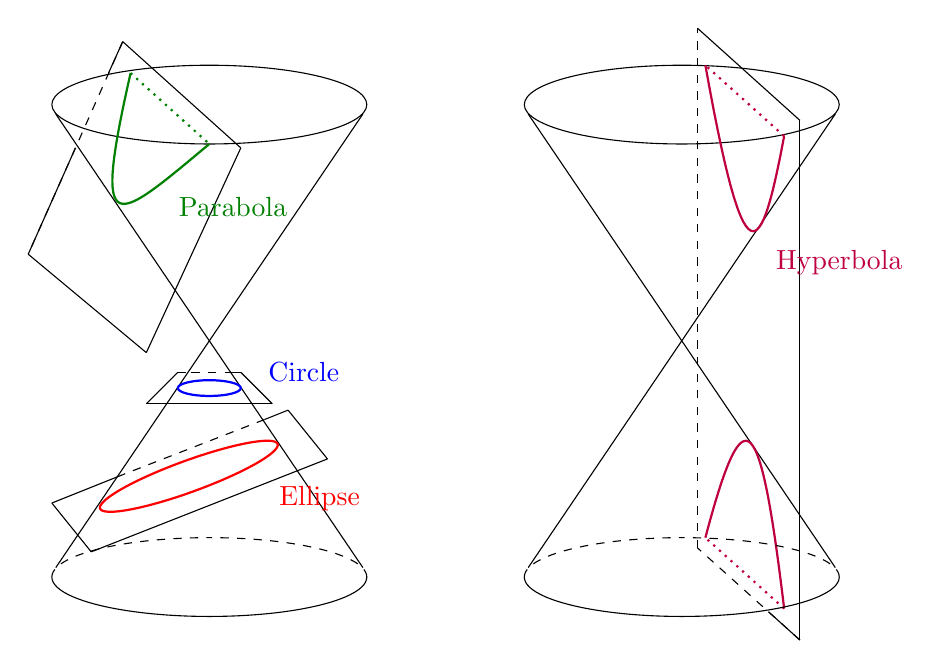
\begin{tikzpicture}
\draw[black] (-3,3) ellipse (2 and 0.5);
\draw[black] (3,3) ellipse (2 and 0.5);
\draw[] (-4.95,2.88) -- (-1.05,-2.88);
\draw[] (-4.95,-2.88) -- (-1.05,2.88);
\draw[] (4.95,2.88) -- (1.05,-2.88);
\draw[] (4.95,-2.88) -- (1.05,2.88);

\draw[blue, thick] (-3,-0.6) ellipse (0.4 and 0.1);
\draw[] (-3.8,-0.8) -- (-2.2,-0.8);
\draw[] (-3.8,-0.8) -- (-3.4,-0.4);
\draw[] (-2.2,-0.8) -- (-2.6,-0.4);
\draw[] (-3.4,-0.4) -- (-3.3,-0.4);
\draw[] (-2.6,-0.4) -- (-2.7,-0.4);
\draw[dashed] (-2.7,-0.4) -- (-3.3,-0.4);
\node[] at (-1.8,-0.4) {\textcolor{blue}{Circle}};

\draw[rotate around={20:(-3.26,-1.72)}, red, thick] (-3.26,-1.72) ellipse (1.2 and 0.2);
\draw[] (-4.5,-2.68) -- (-1.5,-1.5);
\draw[] (-4.5,-2.68) -- (-5,-2.06);
\draw[] (-5,-2.06) -- (-4.1,-1.7);
\draw[] (-1.5,-1.5) -- (-2,-0.88);
\draw[] (-2,-0.88) -- (-2.3,-1);
\draw[dashed] (-2.3,-1) -- (-4.1,-1.7);
\node[] at (-1.6,-2) {\textcolor{red}{Ellipse}};

\draw[Green, thick] (-4,3.4) .. controls (-4.5,1.2) and (-4.2,1.5) .. (-3,2.5);
\draw[dotted, Green, thick] (-4,3.4) -- (-3,2.5);
\draw[] (-2.6,2.45) -- (-3.8,-0.15);
\draw[] (-2.6,2.45) -- (-4.1,3.8) coordinate (A);
\draw[] (-3.8,-0.15) -- (-5.3,1.1) coordinate (B);
\draw[dashed] (A) -- (B);
\draw[] (A) -- (-4.28,3.4);
\draw[] (B) -- (-4.7,2.45);
\node[] at (-2.7,1.7) {\textcolor{Green}{Parabola}};

\draw[] (4.5,-3.8) coordinate (A) -- (4.5,2.8) coordinate (B);
\draw[dashed] (A) -- (3.2,-2.63) coordinate (C);
\draw[] (B) -- (3.2,3.97) coordinate (D);
\draw[dashed] (C) -- (D);
\draw[purple, thick] (4.3,-3.4) coordinate (E) .. controls (4,-0.9) and (3.8,-0.6) .. (3.3,-2.5) coordinate (F);
\draw[dotted, purple, thick] (E) -- (F); 
\draw[purple, thick] (4.3,2.6) coordinate (G) .. controls (4,1) and (3.8,0.7) .. (3.3,3.5) coordinate (H);
\draw[dotted, purple, thick] (G) -- (H); 
\draw[] (A) -- (4.1,-3.44);
\node[] at (5,1) {\textcolor{purple}{Hyperbola}};

\pgfpathmoveto{\pgfpoint{-1cm}{-3cm}}
\pgfpatharcto{2cm}{0.5cm}{0}{0}{0}{\pgfpoint{-3cm}{-3.5cm}}
\pgfpathmoveto{\pgfpoint{-5cm}{-3cm}}
\pgfpatharcto{2cm}{0.5cm}{0}{0}{-1}{\pgfpoint{-3cm}{-3.5cm}}
\pgfstroke

\pgfsetdash{{3pt}{3pt}}{0pt}
\pgfpathmoveto{\pgfpoint{-1cm}{-3cm}}
\pgfpatharcto{2cm}{0.5cm}{0}{0}{-1}{\pgfpoint{-3cm}{-2.5cm}}
\pgfpathmoveto{\pgfpoint{-5cm}{-3cm}}
\pgfpatharcto{2cm}{0.5cm}{0}{0}{0}{\pgfpoint{-3cm}{-2.5cm}}
\pgfstroke

\pgfsetdash{{3pt}{0pt}}{0pt}
\pgfpathmoveto{\pgfpoint{1cm}{-3cm}}
\pgfpatharcto{2cm}{0.5cm}{0}{0}{-1}{\pgfpoint{3cm}{-3.5cm}}
\pgfpathmoveto{\pgfpoint{5cm}{-3cm}}
\pgfpatharcto{2cm}{0.5cm}{0}{0}{0}{\pgfpoint{3cm}{-3.5cm}}
\pgfstroke

\pgfsetdash{{3pt}{3pt}}{0pt}
\pgfpathmoveto{\pgfpoint{1cm}{-3cm}}
\pgfpatharcto{2cm}{0.5cm}{0}{0}{0}{\pgfpoint{3cm}{-2.5cm}}
\pgfpathmoveto{\pgfpoint{5cm}{-3cm}}
\pgfpatharcto{2cm}{0.5cm}{0}{0}{-1}{\pgfpoint{3cm}{-2.5cm}}
\pgfstroke
\end{tikzpicture}\\
(Adapted from the code of Ridlo W. Wibowo)
\end{center}
\begin{defn}[Conic Sections]
\label{defn:conic}
Conic Sections (circles, ellipses, parabola, hyperbola) are the curves generated by a second-degree polynomial in two variables $(x, y)$ that takes the general form of
\begin{align*}
ax^2 + bxy + cy^2 + mx + ny - h = 0
\end{align*}
where $a$, $b$, $c$, $m$, $n$ and $h$ are all constants. It can be expressed as a quadratic form:
\begin{align*}
\textbf{x}^T B\textbf{x} = 
\begin{bmatrix}
x & y & 1
\end{bmatrix}
\begin{bmatrix}
a & \frac{b}{2} & \frac{m}{2} \\
\frac{b}{2} & c & \frac{n}{2} \\
\frac{m}{2} & \frac{n}{2} & -h
\end{bmatrix}
\begin{bmatrix}
x \\
y \\
1
\end{bmatrix} = 0
\end{align*}
where $\textbf{x}^T = (x,y,1)^T$.
\end{defn}
To see what types of conic sections the quadratic form represents, we can examine the determinants of $B$ and its minor $B_{33}$. We simply state the results below.
\begin{proper}
\label{proper:quadgentype}
The quadratic form constructed in Definition \ref{defn:conic} represents a degenerate conic if $\det(B) = 0$. Otherwise, if $\det(B) \neq 0$, it indicates
\begin{itemize}
    \item a hyperbola if $\det(B_{33}) < 0$;
    \item a parabola if $\det(B_{33}) = 0$;
    \item an ellipse if $\det(B_{33}) > 0$.
\end{itemize}
where
\begin{align*}
B_{33} = 
\begin{bmatrix}
a & \frac{b}{2} \\
\frac{b}{2} & c 
\end{bmatrix}
\end{align*}
In the case of an ellipse so that $\det(B_{33}) > 0$, if $a = c$ and $b = 0$, then it is further reduced to a circle.
\end{proper}
However, for simplicity, we will only discuss the \index{Central Conics}\keywordhl{central conics} where the linear terms $mx$ and $ny$ do not appear. This excludes the case of parabola, only keeping the ellipses and hyperbola. The quadratic form then can be simplified as follows.
\begin{proper}
\label{proper:quadcentraltype}
Ellipses (plus circles) and hyperbola, centered at the origin, are called central conics and have the form of
\begin{align*}
ax^2 + bxy + cy^2 = h
\end{align*}
or expressed as a quadratic form of
\begin{align*}
\textbf{x}^T B_{33} \textbf{x} = h
\end{align*}
where now $\textbf{x} = (x,y)^T$ only and $B_{33}$ is as defined in Properties \ref{proper:quadgentype}.
\end{proper}
By Properties \ref{proper:quadgentype}, they can be classified by the discriminant $\Delta = b^2 - 4ac$, which is easily seen to be equal to $-4\det(B_{33})$: The discriminant is positive (negative) when the graph is a hyperbola (ellipse) and $\det(B_{33})$ is negative (positive). A zero discriminant actually represents a "parabola", but the removal of linear terms in the conic section equation reduces the parabola to degenerate straight lines. \par
Short Exercise: Identify the types of curve generated by $x^2 - xy + 2y^2 = 3$ and $x^2 + xy - y^2 = 1$.\footnote{The first one is an ellipse ($\Delta = (-1)^2 - 4(1)(2) = -7 < 0$) and the second one is a hyperbola ($\Delta = (1)^2 - 4(1)(-1) = 5 > 0$).}\par
Notice that sometimes an "ellipse" where $\det(B_{33}) > 0$ may not produce real graph and is imaginary. (Take $x^2 + 2y^2 = -3$ as an example.) To address this, we can link the definiteness property of quadratic forms to arrive at an equivalent classification:
\begin{thm}
\label{thm:quadcentraltypealt}
Given $\textbf{x}^TB_{33}\textbf{x} = h$ as in Properties \ref{proper:quadcentraltype}, where $h$ is chosen to be $1$ for scaling, then it represents
\begin{itemize}
\item an ellipse if $B_{33}$ is positive definite,
\item a hyperbola if $B_{33}$ is indefinite,
\item no real graph if $B_{33}$ is negative definite.
\end{itemize}
\end{thm}
The above works because if the central conic is a hyperbola and $\det(B_{33})$ is negative, then from the view point of orthogonal diagonalization the $2 \times 2$ $B_{33}$ matrix must have one positive and one negative eigenvalue, which by Theorem \ref{thm:quaddefinite} is the same as being indefinite. It is similar for an ellipse where $B_{33}$ being positive-definite means that its two eigenvalues are both positive and $\det(B_{33})$ is positive as well. Meanwhile, when $B_{33}$ is negative-definite, the two eigenvalues are both negative and $\det(B_{33})$ is still positive. Nevertheless, as $h$ is chosen to be $1$, the negative-definiteness means that $\textbf{x}$ has no real solution.
\begin{center}
\begin{tikzpicture}
\draw[thick, ->] (-3,0) -- (3,0) node[right]{$x$};
\draw[thick, ->] (0,-3) -- (0,3) node[above]{$y$};
\draw[Green,rotate=30] plot[domain=-1.2:1.3] ({1*cosh(\x)},{1*sinh(\x)});
\draw[Green,rotate=30] plot[domain=-1.2:1.3] ({-1*cosh(\x)},{1*sinh(\x)});
\draw[red,rotate=30] plot[domain=-3:3] ({\x},{0});
\draw[blue,rotate=-60] plot[domain=-3:3] ({\x},{0});
\end{tikzpicture}
\begin{tikzpicture}
\draw[thick, ->] (-3,0) -- (3,0) node[right]{$x$};
\draw[thick, ->] (0,-3) -- (0,3) node[above]{$y$};
\draw[Green, rotate=-30] (0,0) ellipse (2 and 1);
\draw[red,rotate=-30] plot[domain=-3:3] ({\x},{0});
\draw[blue,rotate=60] plot[domain=-3:3] ({\x},{0});
\end{tikzpicture}
\end{center}
Left: A hyperbola ($x^2 + 2\sqrt{3}xy - y^2 = 1$), Right: An ellipse ($\frac{7}{4}x^2 + \frac{3}{2}\sqrt{3}xy + \frac{13}{4}y^2 = 1$). Both of them are rotated from their standard position so that their major axis (red) and minor axis (blue) are not aligned with the $x$/$y$ axes and make an angle of 30 degrees.\par

For example, the quadratic equation represented by the quadratic form $\textbf{x}^TB\textbf{x} = 1$, where
\begin{align*}
B &=
\begin{bmatrix}
1 & -2 \\
-2 & 3
\end{bmatrix}
\end{align*}
is equivalent to $x^2 - 4xy + 3y^2 = 1$. $B$ can be shown to have an eigenvalue of $\lambda = 2 \pm \sqrt{5}$. As $\lambda_+ = 2 + \sqrt{5} > 0$ and $\lambda_- = 2 - \sqrt{5} < 0$, $B$ is indefinite and the curves are a pair of hyperbola by Theorem \ref{thm:quadcentraltypealt}.\\
\\
The figure in the last page shows that hyperbola and ellipses can be rotated from their standard position. The effect on the resulted quadratic equation by an orthogonal matrix is to produce cross-product terms ($xy$ in two-dimensional cases), which can be eliminated by an inverse rotation to restore the curves so that the major and minor axes are again oriented along the $x$ and $y$ axes. If the graphs start with being tilted by an angle of $\theta$, we can make a rotation by the same angle $\theta$ but in an opposite direction to recover the \textit{standard position}. It is equivalent to rotate the coordinate system by an angle of $\theta$ in the same sense of the initial tilting. The readers can be referred back to Section \ref{section:orthogeometricsub} and Definition \ref{defn:coordtransquad} about the rotation of a coordinate system for a quadratic form.

\begin{exmp}
Rotate the quadratic equation $x^2 - xy + y^2 = 1$ so that the major axis lies along the $x$-axis.
\end{exmp}
First, we cast the equation into the quadratic form $\textbf{x}^T B\textbf{x} = 1$, with
\begin{align*}
B &=
\begin{bmatrix}
1 & -\frac{1}{2} \\
-\frac{1}{2} & 1
\end{bmatrix}
\end{align*}
We first find the eigenvalues of $B$, the characteristic equation is
\begin{align*}
\begin{vmatrix}
1-\lambda & -\frac{1}{2} \\
-\frac{1}{2} & 1-\lambda
\end{vmatrix} = (1-\lambda)^2 - (-\frac{1}{2})^2 &= 0 \\
\lambda^2 - 2\lambda + \frac{3}{4} &= 0 \\
\lambda &= \frac{1}{2} \text{ or } \frac{3}{2}
\end{align*}
So by Theorem \ref{thm:quadcentraltypealt}, $A$ is positive definite and it is an ellipse. The smaller (larger) eigenvalue corresponds to the major (minor) axis. Now we consider an orthogonal matrix $P$ to perform a rotation on the coordinate system, with the old coordinates related to the new coordinates by $\textbf{x} = P\textbf{x}'$. So the quadratic form is transformed to
\begin{align*}
(P\textbf{x}')^T B (P\textbf{x}') &= \textbf{x}'^T (P^T BP) \textbf{x}'
\end{align*}
We immediately identify $P^T BP$ as a rotation of the coordinate system for the matrix $B$, as noted by Definition \ref{defn:coordtransquad}. Section \ref{section:orthogonaldiagreal} tells us that we can deal with the cross-product terms by orthogonal diagonalization, which turns the off-diagonal entries in $B$ into zeros. The normalized eigenvectors of $B$ are found to be
\begin{align*}
&\vec{v}_\lambda = \begin{bmatrix}
\frac{1}{\sqrt{2}} \\
\frac{1}{\sqrt{2}}
\end{bmatrix}
\text{ for } \lambda = \frac{1}{2}
& \begin{bmatrix}
-\frac{1}{\sqrt{2}} \\
\frac{1}{\sqrt{2}}
\end{bmatrix}
\text{ for } \lambda = \frac{3}{2}
\end{align*}
Hence we can set 
\begin{align*}
P =
\begin{bmatrix}
\frac{1}{\sqrt{2}} & -\frac{1}{\sqrt{2}} \\
\frac{1}{\sqrt{2}} & \frac{1}{\sqrt{2}}
\end{bmatrix}
\end{align*}
So that
\begin{align*}
P^T BP = 
\begin{bmatrix}
\frac{1}{\sqrt{2}} & \frac{1}{\sqrt{2}} \\
-\frac{1}{\sqrt{2}} & \frac{1}{\sqrt{2}}
\end{bmatrix}
\begin{bmatrix}
1 & -\frac{1}{2} \\
-\frac{1}{2} & 1
\end{bmatrix}
\begin{bmatrix}
\frac{1}{\sqrt{2}} & -\frac{1}{\sqrt{2}} \\
\frac{1}{\sqrt{2}} & \frac{1}{\sqrt{2}}
\end{bmatrix}
=
\begin{bmatrix}
\frac{1}{2} & 0\\
0 & \frac{3}{2}
\end{bmatrix}
= D
\end{align*}
The new equation is seen to be $\textbf{x}'^T D\textbf{x} = 1$, or $\frac{1}{2}(x')^2 + \frac{3}{2}(y')^2 = 1$. Below are the diagrams before and after the rotation. The major (minor) axis now matches the $x$($y$)-axis as we place the smaller (larger) eigenvalue in the first (second) diagonal entry in $D$.

\begin{center}
\begin{tikzpicture}
\draw[thick, ->] (-3,0) -- (3,0) node[right](vecu){$x$};
\draw[thick, ->] (0,-3) -- (0,3) node[above]{$y$};
\draw[Green, thick, rotate=45] (0,0) ellipse ({1.2*sqrt(2)} and {1.2*sqrt(2/3)});
\draw[red, ->] (0,0) -- (2,2) node[above right](vecv){$x'$, Major axis, $\lambda = 1/2$};
\draw[blue, ->] (0,0) -- (-1,1) node[above left]{$y'$, Minor axis, $\lambda = 3/2$};
\node[Green] at (2,-2) {$x^2 - xy + y^2 = 1$};
\pic[draw, ->, "$45^\circ$", angle eccentricity=1.75] {angle = vecu--0--vecv};
\end{tikzpicture} \\
(Before rotation) \\
\begin{tikzpicture}
\draw[red, thick, ->] (-3,0) -- (3,0) node[right](vecu){$x'$};
\draw[blue, thick, ->] (0,-3) -- (0,3) node[above]{$y'$};
\draw[Green, thick, rotate=0] (0,0) ellipse ({1.2*sqrt(2)} and {1.2*sqrt(2/3)});
\node[Green] at (2,-2) {$\frac{1}{2}(x')^2 + \frac{3}{2}(y')^2 = 1$};
\end{tikzpicture} \\
(After rotation)
\end{center}
The degree of tilting can be found to be exactly $\pi/4 = 45^{\circ}$, by comparing the general two-dimensional rotation matrix
\begin{align*}
\begin{bmatrix}
\cos \theta & -\sin \theta \\
\sin \theta & \cos \theta
\end{bmatrix}
\end{align*}
against $P$. $\cos \theta = \frac{1}{\sqrt{2}}$ and $\sin \theta = \frac{1}{\sqrt{2}}$ implies that $\tan \theta = 1$, and $\theta = \pi/4$. The possibility of eliminating the cross-product terms in quadratic forms is formally known as the \index{Principal Axes Theorem}\keywordhl{Principal Axes Theorem}.

\begin{thm}[Principal Axes Theorem]
For a quadratic form $\textbf{x}^TB\textbf{x}$, where $B$ is a symmetric matrix, we can always make an orthogonal change of variable $\textbf{x}' = P^T\textbf{x}$ (or equivalently $\textbf{x} = P\textbf{x}'$) such that it turns into $\textbf{x}'^TD\textbf{x}' = \lambda_1 x_1'^2 + \lambda_2 x_2'^2 + \cdots$ which contains purely quadratic terms and no cross-product terms. The primed coordinates $\textbf{x}'$ then represent the \textit{principal axes}. $P$ is formed by the set of orthonormal column eigenvectors of $B$ and $D$ is a diagonal matrix with entries being the eigenvalues of $B$.
\end{thm}
This is simply a rephrasing of Definition \ref{defn:orthodiagonal} and Properties \ref{proper:orthobasissym}. In general, for a two-dimensional quadratic form
\begin{align*}
\begin{bmatrix}
a & \frac{b}{2} \\
\frac{b}{2} & c
\end{bmatrix}
\end{align*}
It can undergo a rotation of the coordinate system by an angle $\theta$ such that
\begin{align*}
\begin{bmatrix}
\cos \theta & \sin \theta \\
-\sin \theta & \cos \theta
\end{bmatrix}
\begin{bmatrix}
a & \frac{b}{2} \\
\frac{b}{2} & c
\end{bmatrix}
\begin{bmatrix}
\cos \theta & -\sin \theta \\
\sin \theta & \cos \theta
\end{bmatrix}
=
\begin{bmatrix}
* & 0\\
0 & *
\end{bmatrix}
\end{align*}
the off-diagonal elements become zero. The required $\theta$ is found by expanding the left hand side and equating both sides, which gives
\begin{align*}
-\sin \theta (a \cos\theta + \frac{b}{2}\sin \theta) + \cos\theta (\frac{b}{2} \cos \theta + c\sin \theta) &= 0 \\
\frac{c-a}{2} \sin (2\theta) + \frac{b}{2}\cos(2\theta) &= 0 \\
\cot(2\theta) &= \frac{a-c}{b}
\end{align*}
where we have applied the familiar double angle formulas from the first line to second line.

\subsubsection{Generalizing to the Three-dimensional Space}
Since physically we are living in a three-dimensional world, it is normal to ask if we can extend the idea of geometrically quadratic shapes from two spatial axes to three. This is possible and we only need to modify the $\textbf{x}$ in the quadratic form to encompass the third axis so that $\textbf{x} = (x,y,z)^T$ and $B$ in $\textbf{x}^TB\textbf{x}$ is now a $3 \times 3$ symmetric matrix. Now the quadratic shapes include \textit{ellipsoids} and \textit{hyperboloids}, and the change in coordinates to convert them into the standard position follows the exact same orthogonal diagonalization procedure. We ask the readers to try working with them in Exercise ??.

\section{Statistics with Quadratic Form}

\subsection{Variance and Covariance}
\label{section:variancesec}
One important quantity in the world of Statistics is the \index{Variance}\keywordhl{variance} of a \textit{random variable} or \textit{time-series}. Variance can be viewed as the spread of distribution behind the random variable. Larger the variance, the more disperse the data points are. In Earth Sciences, we often use it to quantify the variability of certain phenomena or patterns, e.g. the variance of spacetime-filtered winds can tell us how active the corresponding wave type is.

\subsubsection{Single Distribution}
We start with the simplest case, the definition of variance for the distribution of a single random variable first. Since in real-life we can only do a finite amount of samplings, the variance of a random variable is always approximated and inferred from the data points if we do not know the underlying statistical distribution.
\begin{defn}
\label{defn:variance}
For a distribution $X$, with $n$ data $x_1, x_2, x_3, \cdots, x_n$, its \index{Population Variance}\keywordhl{population variance} is
\begin{align*}
\sigma^2 = \text{Var}(X) &= \frac{1}{n} ((x_1 - \mu)^2 + (x_2 - \mu)^2 + (x_3 - \mu)^2 + \cdots + (x_n - \mu)^2) \\
&= \frac{1}{n} \sum_{k=1}^n (x_k - \mu)^2
\end{align*}
where $\mu$ is the \index{Mean}\keywordhl{mean}, or \index{Expected Value}\keywordhl{expected value} of $X$, and is computed by
\begin{align*}
\mu = E(X) = \frac{1}{n} (x_1 + x_2 + x_3 + \cdots + x_n)
\end{align*}
that is, the average of all data. Hence, variance is the average of squares of difference between the data and their mean, equivalent to $E((X-\mu)^2)$.
\end{defn}
A simpler formula for computing the population variance is
\begin{align*}
\sigma^2 &= E((X-\mu)^2) \\
&= E((X-E(X))^2) \\
&= E(X^2-2XE(X)+(E(X))^2) \\
&= E(X^2) - 2E(X)E(X) + (E(X))^2 & \begin{aligned}\text{(Note that $E(X)$ is a constant}\\ \text{and $E(E(X)) = E(X)$,} \\
\text{$E(XE(X)) = E(X)E(X)$.)}\end{aligned} \\
&= E(X^2) - (E(X))^2 = E(X^2) - \mu^2
\end{align*}
As said before we always have a finite sample, to account this, sometimes we have to use the sample variance $s^2$, which is the same as population variance but with the $\frac{1}{n}$ factor replaced by $\frac{1}{n-1}$. (Hence $s^2 = \frac{n}{n-1}\sigma^2$.) As an example, given a dataset $X$, with $5$ data $\vec{x} = (1, 3, 6, 9, 11)^T$, then their mean is
\begin{align*}
\mu = \frac{1}{5}(1 + 3 + 6 + 9 + 11) = 6
\end{align*}
and the population variance is
\begin{align*}
\sigma^2 = \frac{1}{5}((1-6)^2 + (3-6)^2 + (6-6)^2 + (9-6)^2 + (11-6)^2) = 13.6
\end{align*}
We can also use the short-cut formula.
\begin{align*}
\sigma^2 &= E(X^2) - \mu^2 \\
&= \frac{1}{5} (1^2 + 3^2 + 6^2 + 9^2 + 11^2) - 6^2 \\
&= 49.6 - 36 \\
&= 13.6
\end{align*}
Short Exercise: Find the sample variance of $X$. \footnote{It is $s^2 = \frac{1}{5-1}((1-6)^2 + (3-6)^2 + (6-6)^2 + (9-6)^2 + (11-6)^2) = 17$. (Or simply compute $\frac{5}{5-1}\sigma^2$.)} \par
Note that the variance formula in Definition \ref{defn:variance} can be written as a dot product shown below.
\begin{proper}
Given a distribution $X$, with $n$ data $\vec{x} = (x_1, x_2, x_3, \cdots, x_n)^T$, and a mean of $\mu$, the population variance can be written as
\begin{align*}
\frac{1}{n} (\vec{x}'\cdot\vec{x}') = \frac{1}{n} \textbf{x}'^T \textbf{x}'
\end{align*}
where $\textbf{x}' = \vec{x}' = \vec{x} - \mu$ is the centered distribution with the mean $\mu$ removed.
\end{proper}
It is simply a matter of observing that $\text{Var}(X) = \frac{1}{n} ((x_1 - \mu)^2 + (x_2 - \mu)^2 + \cdots + (x_n - \mu)^2) = \frac{1}{n} (x_1 - \mu, x_2 - \mu, \ldots, x_n - \mu)^T \cdot (x_1 - \mu, x_2 - \mu, \ldots, x_n - \mu)^T$. Notice that variance, as a sum of squares, can never be negative, and is a positive-semidefinite quantity. \par
Short Exercise: Discuss under what situation the variance will be zero.\footnote{When all data are equal (to the mean).}

\subsubsection{Linear Combination of Multiple Distributions}
Sometimes we may need to consider the "overall" distribution of the sum of multiple variables. More generally, given any linear combination of multiple distributions, like $Z = c_1X^{(1)} + c_2X^{(2)} + \cdots + c_nX^{(n)}$, we may want to know about how to compute its mean and variance. The mean will be simply $\mu_Z = E(c_1 + c_2X^{(2)} + \cdots + c_nX^{(n)}) = c_1E(X^{(1)}) + c_2E(X^{(2)}) + \cdots + c_nE(X^{(n)}) = c_1\mu_1 + c_2\mu_2 + \cdots + c_n\mu_n$, where $E$ is linear and $E(X^{(j)}) = \mu_j$ is the mean of $X^{(j)}$. The variance $\text{Var}(Z)$ is a bit more complicated. First, we need to introduce the concept of \index{Covariance}\keywordhl{covariance} between any two variables, which indicates how they change together.
\begin{defn}
\label{defn:covariance}
For two distributions $X$ and $Y$ consisted of $n$ pairs of data, their population covariance is
\begin{align*}
\text{Cov}(X,Y) &= \frac{1}{n}((x_1-\mu_x)(y_1-\mu_y) + (x_2-\mu_x)(y_2-\mu_y)) \\
&\quad + \cdots + (x_n-\mu_x)(y_n-\mu_y)) \\
&= \frac{1}{n}\sum_{k=1}^{n} (x_k-\mu_x)(y_k-\mu_y)
\end{align*}
where $\mu_x$ and $\mu_y$ are the population means of $X$ and $Y$ respectively. It can be easily seen that $\text{Cov}(X,Y) = \text{Cov}(Y,X)$ so the order does not matter. If $\vec{x}'$ and $\vec{y}'$ are the centered data with their respective mean subtracted away, then their covariance can be denoted by a dot product as
\begin{align*}
\frac{1}{n} \vec{x}' \cdot \vec{y}' = \frac{1}{n} \textbf{x}'^T \textbf{y}'
\end{align*}
For sample covariance, it is
\begin{align*}
q_{xy} = \frac{1}{n-1} \sum_{k=1}^{n} (x_k-\bar{x})(y_k-\bar{y})
\end{align*}
where $\bar{x}$ and $\bar{y}$ are the \textit{sample means} of $X$ and $Y$ which happen to have the same values as $\mu_x$ and $\mu_y$.
\end{defn}
There is also a short-cut formula very similar to that for variance:
\begin{align*}
\text{Cov}(X,Y) &= E((X-E(X))(Y-E(Y))) \\
&= E(XY - E(X)Y - XE(Y) + E(X)E(Y)) \\
&= E(XY) - E(X)E(Y) - E(X)E(Y) + E(X)E(Y) \\
&= E(XY) - E(X)E(Y) 
\end{align*}
In general, if $\text{Cov}(X,Y)$ is positive (negative), it means that when $X$ increases, $Y$ tends to increase (decrease) together. Finally, a direct comparison reveals that $\text{Cov}(X,X) = \text{Var}(X)$ for any distribution $X$. 

\begin{exmp}
Two time-series of measured zonal and meridional wind speed $U$ and $V$ at a weather station, are as shown in the table below.
\begin{center}
\begin{tabular}{|c|c|c|}
\hline
(in \si{\m \per \s}) & $U$ & $V$\\
\hline
1st Measurement & $4.4$ & $-3.5$ \\
\hline
2nd Measurement & $3.8$ & $-2.6$ \\
\hline
3nd Measurement & $3.3$ & $-2.7$ \\
\hline
4th Measurement & $2.8$ & $-1.4$ \\
\hline
5th Measurement & $2.9$ & $-1.2$ \\
\hline
6th Measurement & $1.7$ & $-0.8$ \\
\hline
7th Measurement & $2.1$ & $-1.1$ \\
\hline
\end{tabular}
\end{center}
Find the covariance of $U$ and $V$.
\end{exmp}
\begin{solution}
It is not hard to get $\mu_U = 3.0$ and $\mu_V = -1.9$. By Definition \ref{defn:covariance}, we have
\begin{align*}
\text{Cov}(U,V) &= \frac{1}{7} [(4.4-3.0)((-3.5)-(-1.9))+(3.8-3.0)((-2.6)-(-1.9)) \\
&\quad+(3.3-3.0)((-2.7)-(-1.9))+(2.8-3.0)((-1.4)-(-1.9)) \\
&\quad+(2.9-3.0)((-1.2)-(-1.9))+(1.7-3.0)((-0.8)-(-1.9)) \\
&\quad+(2.1-3.0)((-1.1)-(-1.9))] \\
&= \frac{-5.36}{7} = \SI{-0.77}{\square\m \per \square\s}
\end{align*}
Alternatively, the short-cut formula gives
\begin{align*}
\text{Cov}(U,V) &= E(UV) - \mu_U \mu_V \\
&= \frac{1}{7}[(4.4)(-3.5) + (3.8)(-2.6) + (3.3)(-2.7) + (2.8)(-1.4) \\
&\quad + (2.9)(-1.2) + (1.7)(-0.8) + (2.1)(-1.1)] - (3.0)(-1.9) \\
&= (-6.466) - (-5.7) = \SI{-0.77}{\square\m \per \square\s}
\end{align*}
\end{solution}
There are two take-away observations from the above example. First, if $X$ and $Y$ both have the same unit $a$, then the unit of their covariance, or the variance for each of them individually, will have a unit of $a^2$. If $Y$ has a unit of $b$ instead then their covariance will have a unit of $ab$. Also, covariance can take negative values, which is different from variance which is always non-negative.\par
Another useful measure related to variance and covariance is \index{Correlation}\keywordhl{correlation}. For two distribution $X$ and $Y$, the correlation is defined by the following formula.
\begin{defn}[Correlation]
The correlation of two distributions $X$ and $Y$ is
\begin{align*}
\rho_{xy} &= \frac{\text{Cov}(X,Y)}{\sqrt{\text{Var}(X) \text{Var}(Y)}} \\
&= \frac{\text{Cov}(X,Y)}{\sqrt{\text{Cov}(X,X) \text{Cov}(Y,Y)}}
\end{align*}
where Var and Cov are computed as given in Definitions \ref{defn:variance} and \ref{defn:covariance}.
\end{defn}
Moreover,
\begin{proper}
The correlation between any two distributions $X$ and $Y$ falls in the range between $-1$ and $1$, i.e. $-1 \leq \rho_{xy} \leq 1$.
\end{proper}
\begin{proof}
We can rewrite the correlation using the vector notation for covariance in Definition \ref{defn:covariance}, which gives
\begin{align*}
\rho_{xy} &= \frac{(\vec{x}' \cdot \vec{y}')}{\sqrt{(\vec{x}'\cdot\vec{x}')(\vec{y}'\cdot\vec{y}')}} \\
&= \frac{(\vec{x}' \cdot \vec{y}')}{\sqrt{{\norm{\vec{x}'}}\norm{\vec{y}'}}}
\end{align*}
where $\vec{x}' = \vec{x} - \mu_x$ and $\vec{y}' = \vec{y} - \mu_y$ are centered by removing the mean from the original distributions. Observe that this quantity takes the same form as the one in the Cauchy-Schwarz Inequality (Theorem \ref{thm:CauchySch}), and by that we promptly know that $\abs{\rho_{xy}} \leq 1$.    
\end{proof}

Correlation between two distributions $X$ and $Y$ indicates how their data varies together just like covariance, but normalized by their variances so that it is dimensionless and will not depend on the units used. Therefore, correlation can be considered as a standardized version of covariance that can be compared across different pairs of variables and is more interpretable. If the correlation is positive, then $X$ and $Y$ will generally increase or decrease together. On the other hand, if the correlation is negative, then when one of them increases, one of them will tend to decrease, and vice versa. Higher the magnitude of correlation, stronger the \textit{linear} relationship. Notice the word "linear" here. If the correlation is close to zero, it simply means that there is no clear linear relationship between them, but this does not exclude the possibility of having other relationships, e.g. exponential or quadratic.\par
In the last example, $\text{Cov}(U,V) = \SI{-0.77}{\square\m \per \square\s}$, $\text{Var}(U) = \SI{0.75}{\square\m \per \square\s}$, $\text{Var}(V) = \SI{0.90}{\square\m \per \square\s}$, and $\rho_{uv} = \frac{-0.77}{\sqrt{(0.75)(0.90)}} \approx -0.94$. We have used the population variance and covariance for the computation, but they can be replaced by the sample counterparts. It may be tempting to claim that a strong negative relationship exists in this case, however, the sample size here is a bit small for this result to be meaningful. \par
Short Exercise: When will $\rho_{xy}$ take the value of $1$ (or $-1$)?\footnote{It will happen if $X$ and $Y$ have a perfect linear positive (negative) relationship so they appear as a straight line $Y = aX + b$ on the $xy$-plane, $a > 0$ ($a < 0$).}\par

We are now prepared to derive the variance formula for linear combinations of multiple variables.
\begin{proper}
\label{proper:variancemul}
For a distribution stemmed from a linear combination of multiple random variables, in the form of $Z = c_1X^{(1)} + c_2X^{(2)} + \cdots + c_nX^{(n)}$, where the coefficients $\vec{c} = (c_1, c_2, \cdots, c_n)^T$ are all constants, the population variance $\text{Var}(Z)$ can be expressed as a quadratic form $\vec{c}^TQ\vec{c}$, where
\begin{align*}
Q &=
\begin{bmatrix}
\text{Cov}(X^{(1)}, X^{(1)}) & \text{Cov}(X^{(1)}, X^{(2)}) & \cdots & \text{Cov}(X^{(1)}, X^{(n)}) \\
\text{Cov}(X^{(2)}, X^{(1)}) & \text{Cov}(X^{(2)}, X^{(2)}) & \cdots & \text{Cov}(X^{(2)}, X^{(n)}) \\
\vdots & \vdots &  & \vdots \\
\text{Cov}(X^{(n)}, X^{(1)}) & \text{Cov}(X^{(n)}, X^{(2)}) & \cdots & \text{Cov}(X^{(n)}, X^{(n)}) \\
\end{bmatrix} \\
&=
\begin{bmatrix}
\text{Var}(X^{(1)}) & \text{Cov}(X^{(1)}, X^{(2)}) & \cdots & \text{Cov}(X^{(1)}, X^{(n)}) \\
\text{Cov}(X^{(2)}, X^{(1)}) & \text{Var}(X^{(2)}) & \cdots & \text{Cov}(X^{(2)}, X^{(n)}) \\
\vdots & \vdots &  & \vdots \\
\text{Cov}(X^{(n)}, X^{(1)}) & \text{Cov}(X^{(n)}, X^{(2)}) & \cdots & \text{Var}(X^{(n)}) \\
\end{bmatrix} 
\end{align*}
is the so-called \index{Covariance Matrix}\keywordhl{covariance matrix} so that $Q_{ij} = \text{Cov}(X^{(i)}, X^{(j)})$. If $[X'] = [X'^{(1)}|X'^{(2)}|\cdots|X'^{(n)}]$ is the matrix consisted of the centered variables $X'^{(j)} = X^{(j)} - E(X^{(j)})$ in columns, then we have $Q = \frac{1}{n}[X']^T[X']$.
\end{proper}
\begin{proof}
Let's say we have $m$ data for $Z$: $z_1, z_2, \ldots, z_m$. Denote the mean of $X^{(j)}$ by $\mu_{j}$. Starting from the expression in Definition \ref{defn:variance}, we have
\begin{align*}
\text{Var}(Z) &= \frac{1}{m} \sum_{k=1}^m (z_k - \mu_z)^2 \\
&= \frac{1}{m} \sum_{k=1}^m (\sum_{j=1}^{n} c_jx^{(j)}_k - \sum_{j=1}^{n} c_j\mu_{j})^2  \\
&= \frac{1}{m} \sum_{k=1}^m (\sum_{j=1}^{n} (c_jx^{(j)}_k - c_j\mu_{j}))^2 \\
&= \frac{1}{m} \sum_{k=1}^m [(\sum_{i=1}^{n} c_i(x^{(i)}_k - \mu_{i}))(\sum_{j=1}^{n} c_j(x^{(j)}_k - \mu_{j}))]  \\
&\quad \text{(Changing to a new dummy summation variable)} \\
&= \frac{1}{m} \sum_{k=1}^m (\sum_{i=1}^{n}\sum_{j=1}^{n} c_ic_j (x^{(i)}_k - \mu_{i})(x^{(j)}_k - \mu_{j})) \\
&= \sum_{i=1}^{n}\sum_{j=1}^{n} c_ic_j (\frac{1}{m} \sum_{k=1}^m (x^{(i)}_k - \mu_{i})(x^{(j)}_k - \mu_{j})) \\
&\quad \text{(Switching the order of summation)} \\
&= \sum_{i=1}^{n}\sum_{j=1}^{n} c_ic_j\text{Cov}(X^{(i)}, X^{(j)}) \quad \text{(Definition \ref{defn:covariance})} \\
&= \vec{c}^T Q\vec{c}
\end{align*}
\end{proof}
For two variables situation, it reduces to
\begin{align*}
\vec{c}^TQ\vec{c} =
\begin{bmatrix}
c_1 & c_2
\end{bmatrix}
\begin{bmatrix}
\text{Cov}(X^{(1)}, X^{(1)}) & \text{Cov}(X^{(1)}, X^{(2)}) \\
\text{Cov}(X^{(2)}, X^{(1)}) & \text{Cov}(X^{(2)}, X^{(2)}) 
\end{bmatrix}
\begin{bmatrix}
c_1 \\
c_2
\end{bmatrix}
\end{align*}

\begin{exmp}
From the previous wind speed observations example, if $W = 0.8U-0.6V$, find $\text{Var}(W)$.
\end{exmp}
\begin{solution}
Earlier calculations show $\text{Var}(U) = \SI{0.75}{\square\m \per \square\s}$,
$\text{Var}(V) = \SI{0.90}{\square\m \per \square\s}$, $\text{Cov}(U,V) = \text{Cov}(V,U) = \SI{-0.77}{\square\m \per \square\s}$. Inserting the values for the expression in Properties \ref{proper:variancemul}, we have
\begin{align*}
\text{Var}(W) &=
\begin{bmatrix}
c_u & c_v
\end{bmatrix}
\begin{bmatrix}
\text{Var}(U) & \text{Cov}(U,V) \\
\text{Cov}(U,V) & \text{Var}(V)
\end{bmatrix}
\begin{bmatrix}
c_u \\
c_v
\end{bmatrix} \\
&=
\begin{bmatrix}
0.8 & -0.6
\end{bmatrix}
\begin{bmatrix}
0.75 & -0.77 \\
-0.77 & 0.90
\end{bmatrix}
\begin{bmatrix}
0.8 \\
-0.6
\end{bmatrix} \\
&= \SI{1.54}{\square\m \per \square\s}
\end{align*} 
\end{solution}
Finally, recall that variance is always a positive-semidefinite quantity, and since it can be calculated as a quadratic form made by the covariance matrix according to Properties \ref{proper:variancemul}, any covariance matrix will also be a positive-semidefinite quadratic form.

\subsection{Principal Component Analysis (PCA)}
A common practice in Earth Science, as well as the growing field of Machine Learning, is to compress the dimensions of a large dataset having many variables/features (\textit{dimensionality reduction}). Given a high number of variables (for example, concentrations of various biochemical substances like blood cells or ions in the blood samples of some hospital patients) in measurements, we want to process them to extract and retain the most important patterns or signals. \index{Principal Component Analysis}\keywordhl{Principal Component Analysis (PCA)}, which also known as \index{Empirical Orthogonal Functions}\keywordhl{Empirical Orthogonal Functions (EOFs)} in Atmospheric Sciences, is the most common technique for this purpose, by finding the mode, or more precisely, the linear combination of features, which maximizes the variance of the data along that direction. \\
\\
Consider the simplest case with two variables, or time-series $X$ and $Y$ first. Assume they have $n$ pairs of data, from $\textbf{x}_1^T = (x_1, y_1)^T$ to $\textbf{x}_n^T = (x_{n}, y_{n})^T$. We can compute the covariance matrix
\begin{align*}
Q = \begin{bmatrix}
\text{Cov}(X, X) & \text{Cov}(X, Y) \\
\text{Cov}(Y, X) & \text{Cov}(Y, Y) 
\end{bmatrix}
\end{align*}
introduced in the last section. Principal Component Analysis sets out to find a unit vector $\textbf{e}$, so that the variance of data projected onto the direction indicated by $\textbf{e}$, which is $\textbf{e}^T Q \textbf{e}$ following from Properties \ref{proper:variancemul}, is maximized.
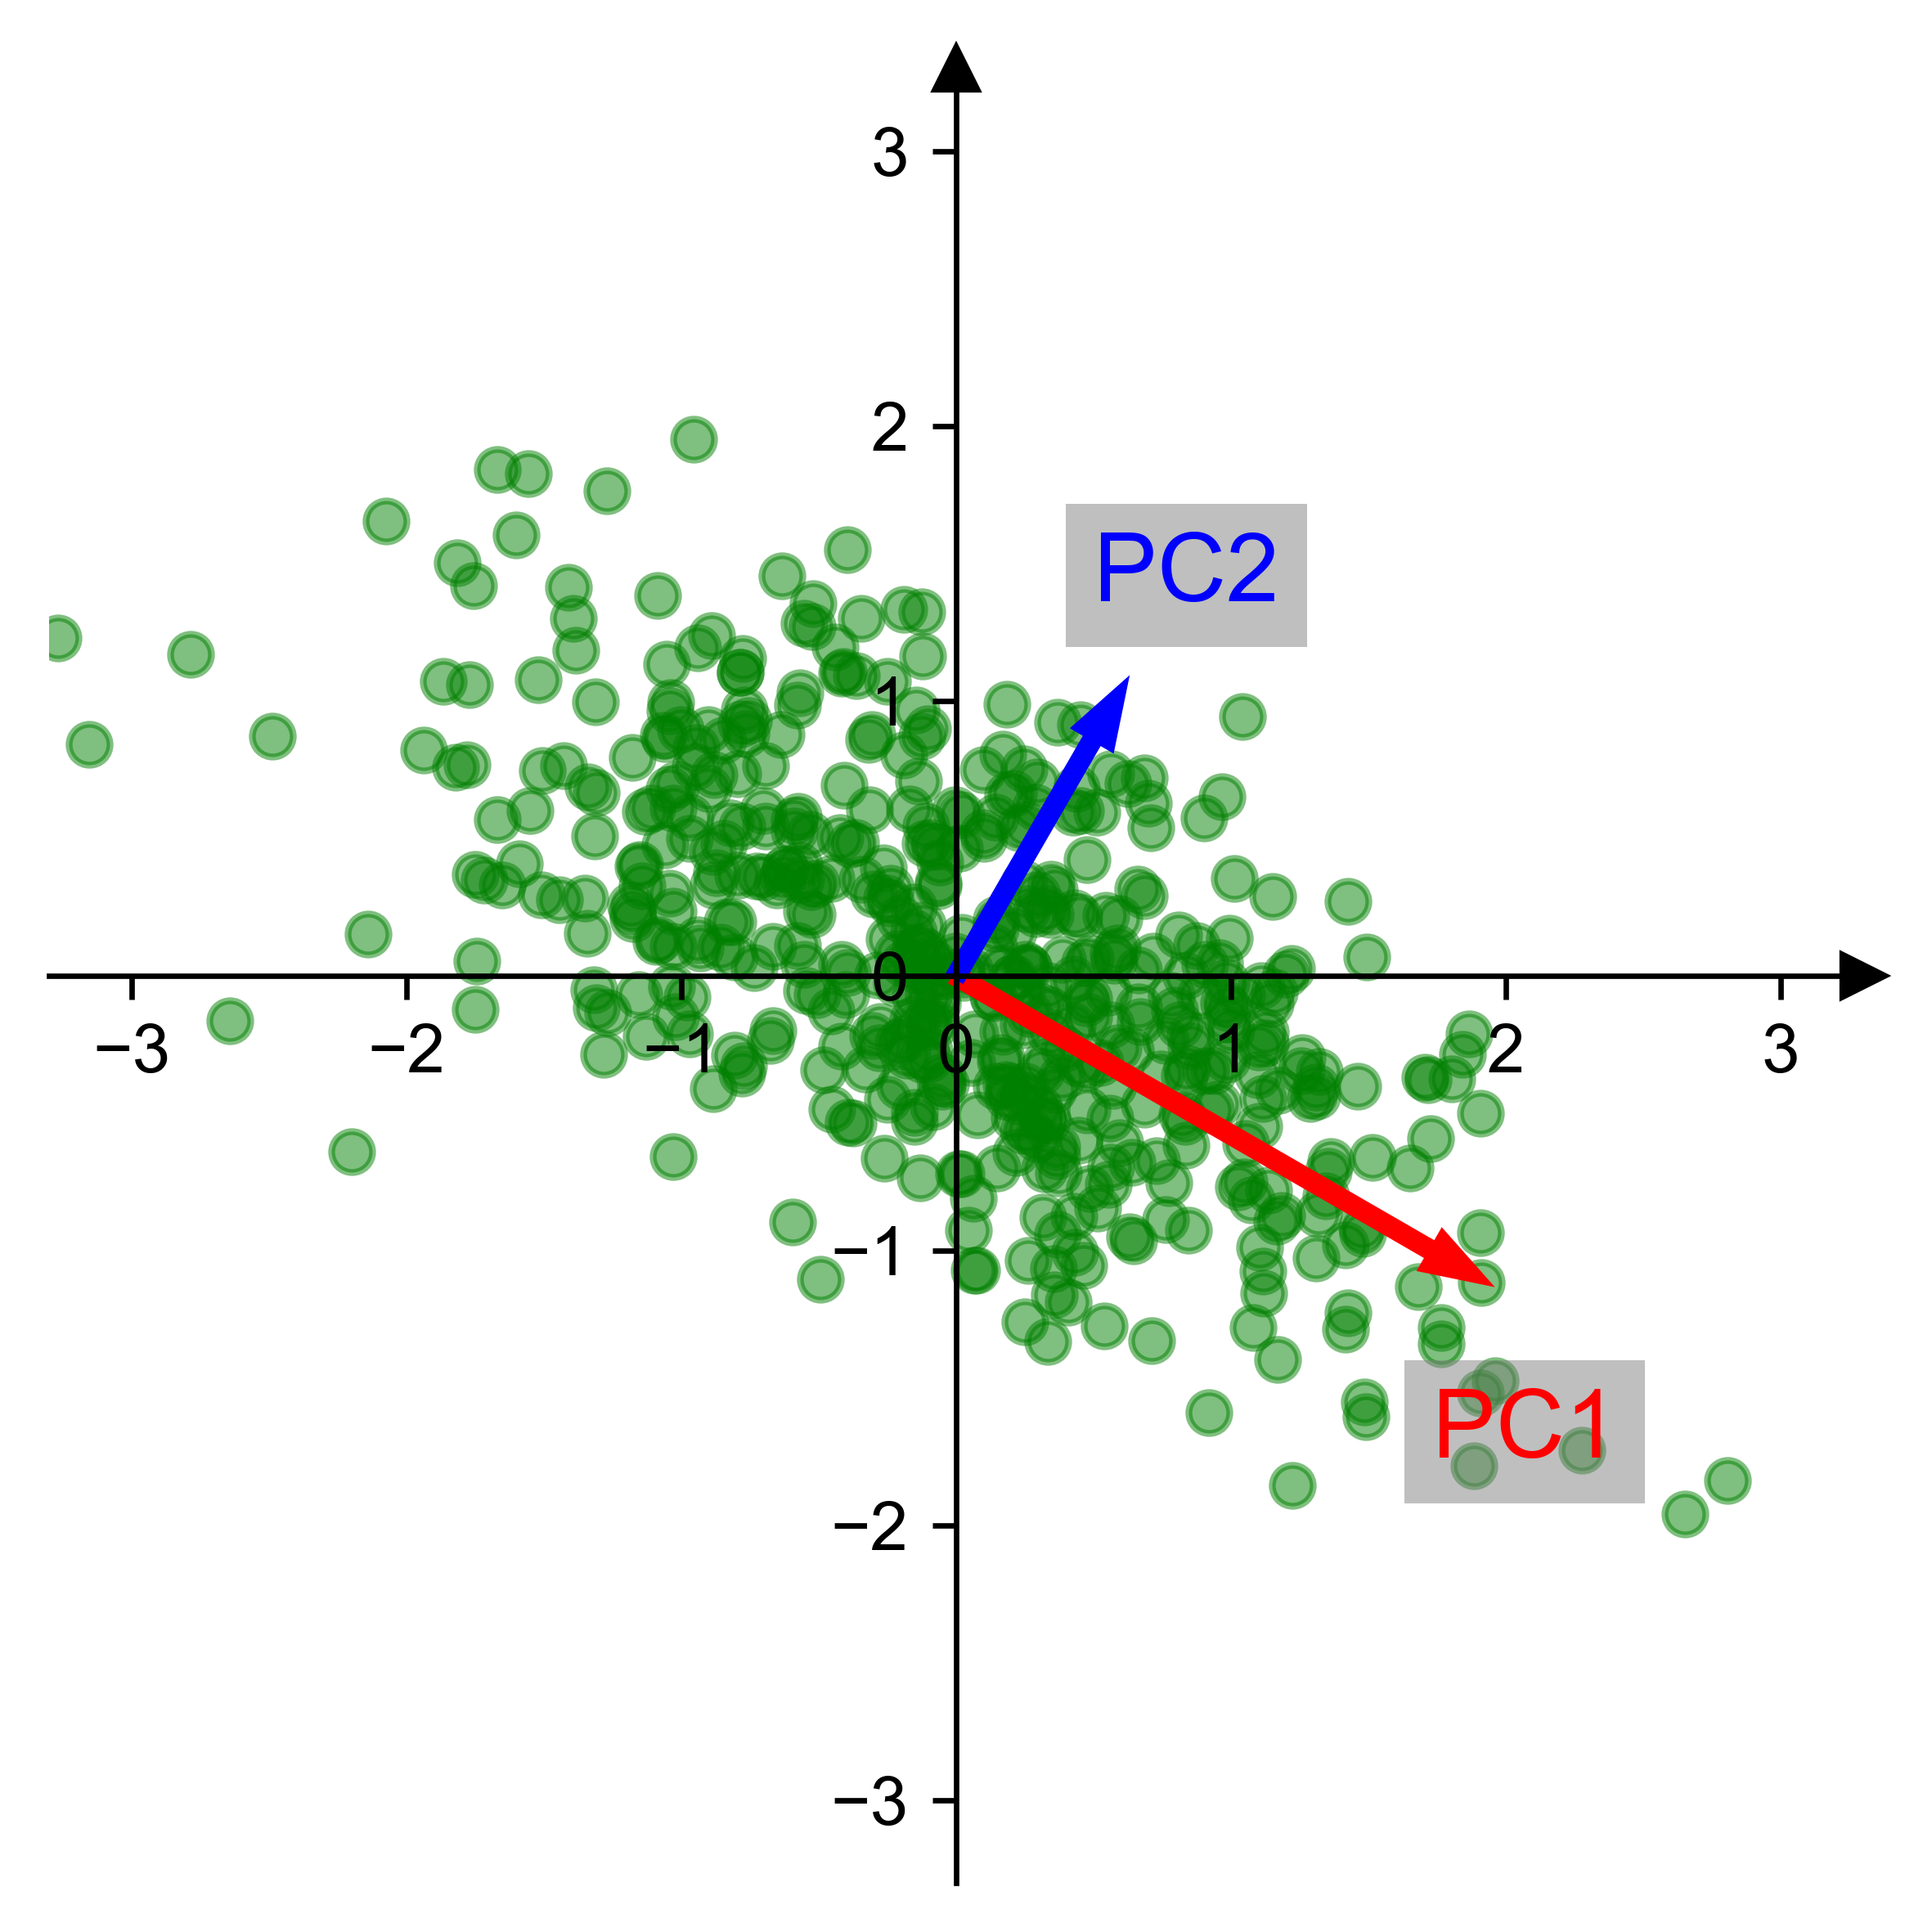
\includegraphics{graphics/PCA_first_demo.png}\\
The two \textit{principal axes/directions} (PCs) found by Principal Component Analysis for a set of data (green). The longer, red (shorter, blue) arrow represents the direction of largest (smallest) variance. The data points can be seen to spread more (less) along that direction. \par
Now the problem is to find, under what situation $\textbf{e}^T Q \textbf{e}$ will assume its largest value. Here, we introduce a famous technique, called \index{Lagrange Multiplier}\keywordhl{Lagrange Multiplier}, coming from elementary Calculus. We will proceed with the case of two variables for brevity.
\begin{thm}[Lagrange Multiplier]
\label{thm:LagrangeMul}
To find the extremal values attained by a function $f(u,v,\cdots)$, under the constraint $g(u,v,\cdots) = 0$, we consider the expression
\begin{align*}
h(u,v,\cdots) = f(u,v,\cdots) - \lambda g(u,v,\cdots)
\end{align*}
where $\lambda$ is a constant so that the system below has a solution:
\begin{align*}
\begin{cases}
\partial h/\partial u &= 0 \\
\partial h/\partial v &= 0 \\
\vdots &= 0
\end{cases}
\end{align*}
$\partial/\partial u$ ($\partial/\partial v$) means differentiating with respect to $u$ ($v$) only while treating other variables as constants. The values of $u$ and $v$ (as well as other variables) required to attain the extremums for $f$ are determined by solving the system of equations above. 
\end{thm}
We are now going to find the value of $x'$ and $y'$ so that $\textbf{e}^T Q \textbf{e}$ obtains the maximum for $\textbf{e}^T = (x',y')$. The constraint is that $\textbf{e}$ is a unit vector as a direction, and hence by the method of Lagrange Multiplier outlined above, we have
\begin{align*}
g(x',y') = x'^2 + y'^2 - 1 = 0
\end{align*}
and with $f(x',y') = \textbf{e}^T Q \textbf{e}$
\begin{align*}
h(x',y') &= (\textbf{e}^T Q \textbf{e}) - \lambda(x'^2 + y'^2 - 1) \\
&= \begin{bmatrix}
x' & y' \\
\end{bmatrix}
\begin{bmatrix}
\text{Cov}(X, X) & \text{Cov}(X, Y) \\
\text{Cov}(Y, X) & \text{Cov}(Y, Y) 
\end{bmatrix}
\begin{bmatrix}
x' \\
y'
\end{bmatrix}
- \lambda(x'^2 + y'^2 - 1) \\
&= x'^2 \text{Cov}(X, X) + 2x'y' \text{Cov}(X, Y) + y'^2\text{Cov}(Y, Y) - \lambda(x'^2 + y'^2 - 1)
\end{align*}
according to Properties \ref{proper:variancemul}. Carrying out the differentiation gives
\begin{align*}
\begin{cases}
\partial h/\partial x' &= 2x'\text{Cov}(X, X) + 2y'\text{Cov}(X, Y) - 2\lambda x' = 0 \\
\partial h/\partial y' &= 2x'\text{Cov}(X, Y) + 2y'\text{Cov}(Y, Y) - 2\lambda y' = 0
\end{cases}    
\end{align*}
This system can be immediately be simplified and recognised as
\begin{align*}
2 \begin{bmatrix}
\text{Cov}(X, X)-\lambda & \text{Cov}(X, Y) \\
\text{Cov}(Y, X) & \text{Cov}(Y, Y)-\lambda
\end{bmatrix}
\begin{bmatrix}
x' \\
y'
\end{bmatrix} &= 0\\
(Q-\lambda I)\textbf{e} &= 0
\end{align*}
which is an eigenvalue problem as introduced in Section \ref{section:eigensection}. Hence we conclude that $f(x',y') = \textbf{e}^T Q \textbf{e}$ can attain an extremal value when $\textbf{e}^T = (x',y')^T$ is a unit eigenvector of $Q$. Notice that since $Q$ is a symmetric matrix, the eigenvectors of $Q$ form an orthonormal basis and are orthogonal to each other by Properties \ref{proper:orthobasissym}. The corresponding magnitude of variance ${\textbf{e}^{(j)}T} Q \textbf{e}^{(j)}$ for the $j$-th eigenvector is
\begin{align*}
{\textbf{e}^{(j)}T} (Q \textbf{e}^{(j)}) &= {\textbf{e}^{(j)}T} (\lambda_j \textbf{e}^{(j)}) \\
&= \lambda_j ({\textbf{e}^{(j)}T} \textbf{e}^{(j)}) \\
&= \lambda_j \norm{\textbf{e}^{(j)}} \\
&= \lambda_j 
\end{align*}
where we have used the facts that $Q \textbf{e}^{(j)} = \lambda_j \textbf{e}^{(j)}$ as per Definition \ref{defn:eigen} and the length of a unit vector is $1$. This means that the variance along the direction of eigenvector is exactly equal to the corresponding eigenvalue. Note that orthogonal diagonalization (see the discussion below Definition \ref{defn:coordtransquad}) transforms the quadratic form to a diagonal matrix consisted of the eigenvalues $\lambda_j$, with respect to the coordinate system made up of the orthonormal eigenvectors $\textbf{e}^{(j)}$. Therefore, from this perspective we can come to the same conclusion that the variance of a transformed variable along the direction indicated by each eigenvector is equal to its eigenvalue, and further, the covariance between two orthogonal directions represented by any pair of distinct eigenvectors are zero, and hence the transformed variables are made uncorrelated. 
\begin{thm}[Principal Component Analysis]
For a covariance matrix $Q$ (which happens to be symmetric), the variance $\textbf{e}^T Q \textbf{e}$ achieves its maximum value $\lambda_1$ along the direction $\textbf{e}^{(1)}$, the largest eigenvalue of $Q$ and the associated unit eigenvector. Generalizing, as $Q$ has $n$ orthonormal eigenvectors $\textbf{e}^{(1)}, \textbf{e}^{(2)}, \cdots, \textbf{e}^{(n)}$, arranged by the magnitude of corresponding eigenvalues $\lambda_1 > \lambda_2 > \cdots > \lambda_n$ from largest to smallest, the largest variance will be $\lambda_1$ when the direction is along $\textbf{e}^{(1)}$, the second largest will be $\lambda_2$ for $\textbf{e}^{(2)}$ and so on, with the smallest variance being $\lambda_n$ for $\textbf{e}^{(n)}$. This set of orthonormal eigenvectors are called the \index{Principal Axes}\index{Principal Directions}\keywordhl{principal axes/directions} in Principal Component Analysis.
\end{thm}
As a side note, any quadratic form $\textbf{e}^TB\textbf{e}$ will attain its maximum and minimum when $\textbf{e}$ is the eigenvector that represents the largest and smallest eigenvalue, which will also be the value that $\textbf{e}^TB\textbf{e}$ takes when it happens. As before, this is under the constraint that $\textbf{e}$ is a unit vector, and this result bears the name of \textit{Constrained Extremum Theorem}.\par
Going back to the problem of Principal Component Analysis, for each principal direction $\textbf{e}^{(j)}$ and the variance $\lambda_{j}$, we can compute the ratio of \index{Explained Variance}\keywordhl{explained variance}, which is the fraction of  $\lambda_{j}$ over the total variance, the sum of eigenvalues/variances from all eigenvectors for the covariance matrix. This quantity allows us to access how well the principal direction contributes to the total variance. In the coordinate system constructed by the orthonormal eigenvectors of $Q$, $[\textbf{e}] = [\textbf{e}^{(1)}|\textbf{e}^{(2)}|\cdots|\textbf{e}^{(n)}]$, the new coordinates for any data point are $\vec{u}_i = [\textbf{e}]^T \vec{x}_i$ (see Section \ref{section:orthogeometricsub}). By the Spectral Theorem \ref{thm:spectral}, this $\vec{u}_i$ can be regarded to be the projection of $\vec{x_i}^T = (x_i, y_i)^T$, the $i$-th pair of data, onto the principal directions and are called the \index{Principal Components}\keywordhl{principal components (PCs)}. \par
Usually, at the start of PCA we will detrend the data and remove the mean from each variable, such that $x'_i = x_i - \bar{x}$ and $y'_i = y_i - \bar{y}$ are used to replace $x_i$ and $y_i$. This enables us to express the covariance matrix as $Q = \frac{1}{n}[X'|Y']^T[X'|Y']$ following the end remark of Properties \ref{proper:variancemul}. 
\begin{exmp}
\label{exmp:tempPCA}
The temperature data of two cities $M$ and $N$ are as follows.
\begin{center}
\begin{tabular}{|c|c|c|c|c|c|}
\hline
(in \si{\degree C}) & $M$ & $N$ & & $M$ & $N$ \\
\hline
1st Day & 21.6 & 22.3 & 8th Day & 22.1 & 22.4 \\
\hline
2nd Day & 21.8 & 21.6 & 9th Day & 21.5 & 21.7 \\
\hline
3nd Day & 20.9 & 21.2 & 10th Day & 22.8 & 22.5 \\
\hline
4th Day & 21.6 & 21.7 & 11th Day & 22.2 & 21.6 \\
\hline
5th Day & 23.4 & 23.2 & 12th Day & 23.0 & 23.3 \\
\hline 
6th Day & 24.7 & 24.1 & 13th Day & 24.2 & 24.7 \\
\hline 
7th Day & 22.0 & 23.9 & 14th Day & 23.8 & 23.1 \\
\hline
\end{tabular}
\end{center}
Perform Principal Component Analysis over them and find the most important principal direction, and extract the time-series of the corresponding PC.
\end{exmp}
\begin{solution}
The means of $M$ and $N$ are $\SI{22.5}{\degree C}$ and $\SI{22.6}{\degree C}$ respectively. After detrending by subtracting the respective means, the new data are
\begin{center}
\begin{tabular}{|c|c|c|c|c|c|}
\hline
(in \si{\degree C}) & $M'$ & $N'$ & & $M'$ & $N'$ \\
\hline
1st Day & -1.5 & -0.3 & 8th Day & -0.4 & -0.2 \\
\hline
2nd Day & -0.7 & -1.0 & 9th Day & -1.0 & -0.9 \\
\hline
3nd Day & -1.6 & -1.4 & 10th Day & 0.3 & -0.1 \\
\hline
4th Day & -0.9 & -0.9 & 11th Day & -0.3 & -1.0 \\
\hline
5th Day & 0.9 & 0.6 & 12th Day & 0.5 & 0.7 \\
\hline 
6th Day & 2.2 & 1.5 & 13th Day & 1.7 & 2.1 \\
\hline 
7th Day & -0.5 & 0.4 & 14th Day & 1.3 & 0.5 \\
\hline
\end{tabular}
\end{center}
From Properties \ref{proper:variancemul}, the sample covariance matrix is
\begin{align*}
Q &= 
\frac{1}{14-1}
\begin{bmatrix}
M' \cdot M' & M' \cdot N' \\
N' \cdot M' & N' \cdot N' 
\end{bmatrix} \\
&= \frac{1}{13}
\begin{bmatrix}
-1.5 & -0.7 & -1.6 & \cdots \\
-0.3 & -1.0 & -1.4 
\end{bmatrix}
\begin{bmatrix}
-1.5 & -0.3 \\
-0.7 & -1.0 \\
-1.6 & -1.4 \\
\vdots
\end{bmatrix} \\
&= \frac{1}{13}
\begin{bmatrix}
18.18 & 13.66 \\
13.66 & 13.64
\end{bmatrix} = 
\begin{bmatrix}
1.398 & 1.051 \\
1.051 & 1.049
\end{bmatrix}
\end{align*}
The unit eigenvectors for $Q$ and thus the principal directions can be found to be $\textbf{e}^{(1)} = (0.763, 0.647)^T$ with a larger variance $\lambda_1 = \SI{2.289}{\square {(\degree C)}}$, and $\textbf{e}^{(2)} = (-0.647, 0.763)^T$ of a smaller variance $\lambda_2 = \SI{0.159}{\square {(\degree C)}}$. The first principal component accounts for $\frac{2.289}{2.289+0.159} \approx 93.5\%$ of the total variance.\\
\\
We can project every pair of data $\vec{x}'^T_i = (m'_i, n'_i)^T$ onto the principal directions by computing $\vec{u}_i = [\textbf{e}]^T\vec{x}'_i$, where $[\textbf{e}] = [\textbf{e}^{(1)}|\textbf{e}^{(2)}]$. The resulting principal components time-series are 
\begin{center}
\begin{tabular}{|c|c|c|c|c|c|c|c|}
\hline
 & D-1 & D-2 & D-3 & D-4 & D-5 & D-6 & D-7 \\
\hline
$u^{(1)}$ & -1.338 & -1.181 & -2.126 & -1.268 & 1.075 & 2.648 & -0.123 \\
\hline
$u^{(2)}$ & 0.741 & -0.310 & -0.034 & -0.105 & -0.124 & -0.278 & 0.628 \\
\hline
 & D-8 & D-9 & D-10 & D-11 & D-12 & D-13 & D-14 \\
\hline
$u^{(1)}$ & -0.434 & -1.345 & 0.164 & -0.875 & 0.834 & 2.655 & 1.315 \\
\hline
$u^{(2)}$ & 0.106 & -0.040 & -0.270 & -0.569 & 0.211 & 0.503 & -0.459 \\
\hline
\end{tabular}
\end{center}
In details, the two principal components for the first day is computed by
\begin{align*}
\begin{bmatrix}
u_1^{(1)} \\
u_1^{(2)} 
\end{bmatrix}
=
\begin{bmatrix}
0.763 & 0.647 \\
-0.647 & 0.763
\end{bmatrix}
\begin{bmatrix}
-1.5 \\
-0.3
\end{bmatrix}
=
\begin{bmatrix}
-1.338\\
0.741
\end{bmatrix}
\end{align*}
The original (detrended) data can be recovered by $\vec{x}'_i = [\textbf{e}]\vec{u}'_i$. If we want to extract the signal originated from the first principal direction only, we can simply remove other column eigenvector(s) in $[\textbf{e}]$ as well as discard the other principal value(s) in $\vec{u}'_i$. The time-series reconstructed by the first PC mode is hence computed by $x'_i = \textbf{e}^{(1)}u_i^{(1)}$:
\begin{center}
\begin{tabular}{|c|c|c|c|c|c|c|c|}
\hline
(in \si{\degree C}) & D-1 & D-2 & D-3 & D-4 & D-5 & D-6 & D-7 \\
\hline
M' & -1.021 & -0.901 & -1.622 & -0.968 & 0.820 & 2.020 & -0.094 \\
\hline
N' & -0.865 & -0.763 & -1.374 & -0.820 & 0.695 & 1.712 & -0.079 \\
\hline
 & D-8 & D-9 & D-10 & D-11 & D-12 & D-13 & D-14 \\
\hline
M' & -0.331 & -1.026 & 0.125 & -0.668 & 0.636 & 2.025 & 1.003 \\
\hline
N' & -0.281 & -0.869 & 0.106 & -0.566 & 0.539 & 1.716 & 0.850 \\
\hline
\end{tabular}
\end{center}
For example, for the third day PC1 contributes
\begin{align*}
x'_3 =
\begin{bmatrix}
m'_3 \\
n'_3
\end{bmatrix}
=
\textbf{e}^{(1)}u_3^{(1)}
=
\begin{bmatrix}
0.763 \\
0.647
\end{bmatrix}
\begin{bmatrix}
-2.126
\end{bmatrix}
=
\begin{bmatrix}
-1.622 \\
-1.374  
\end{bmatrix}
\end{align*}
\begin{center}
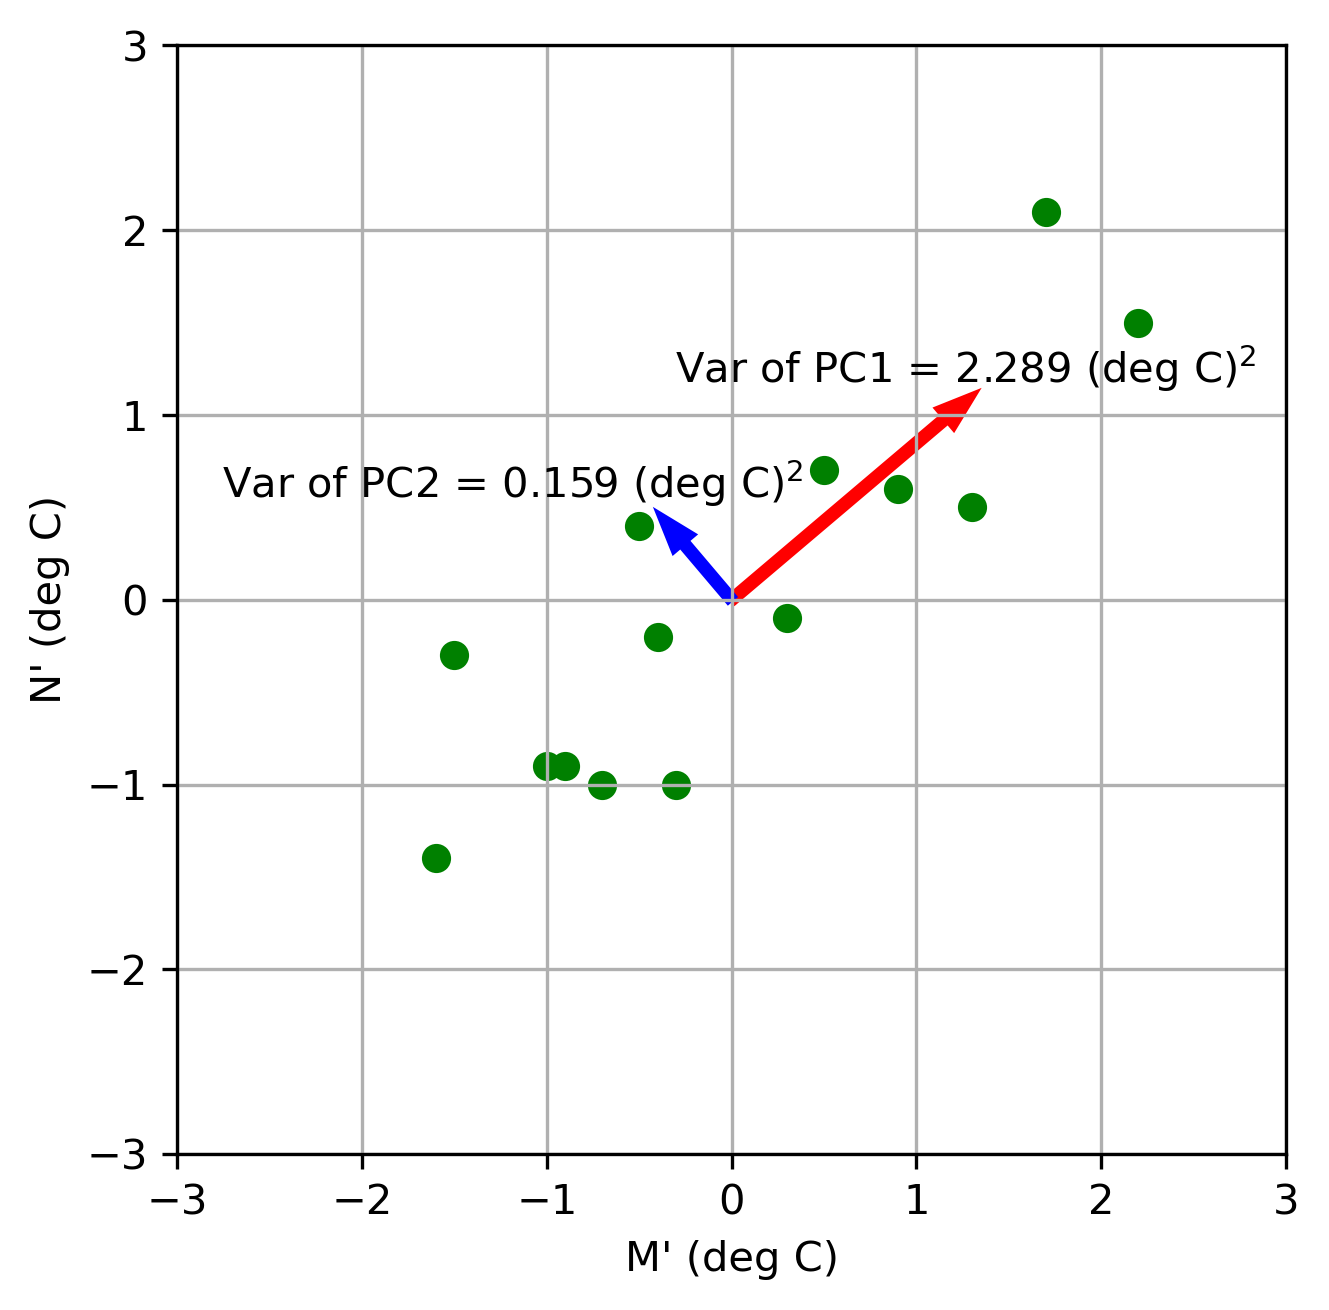
\includegraphics[scale = 0.75]{graphics/PCA_exmp_1.png}\\
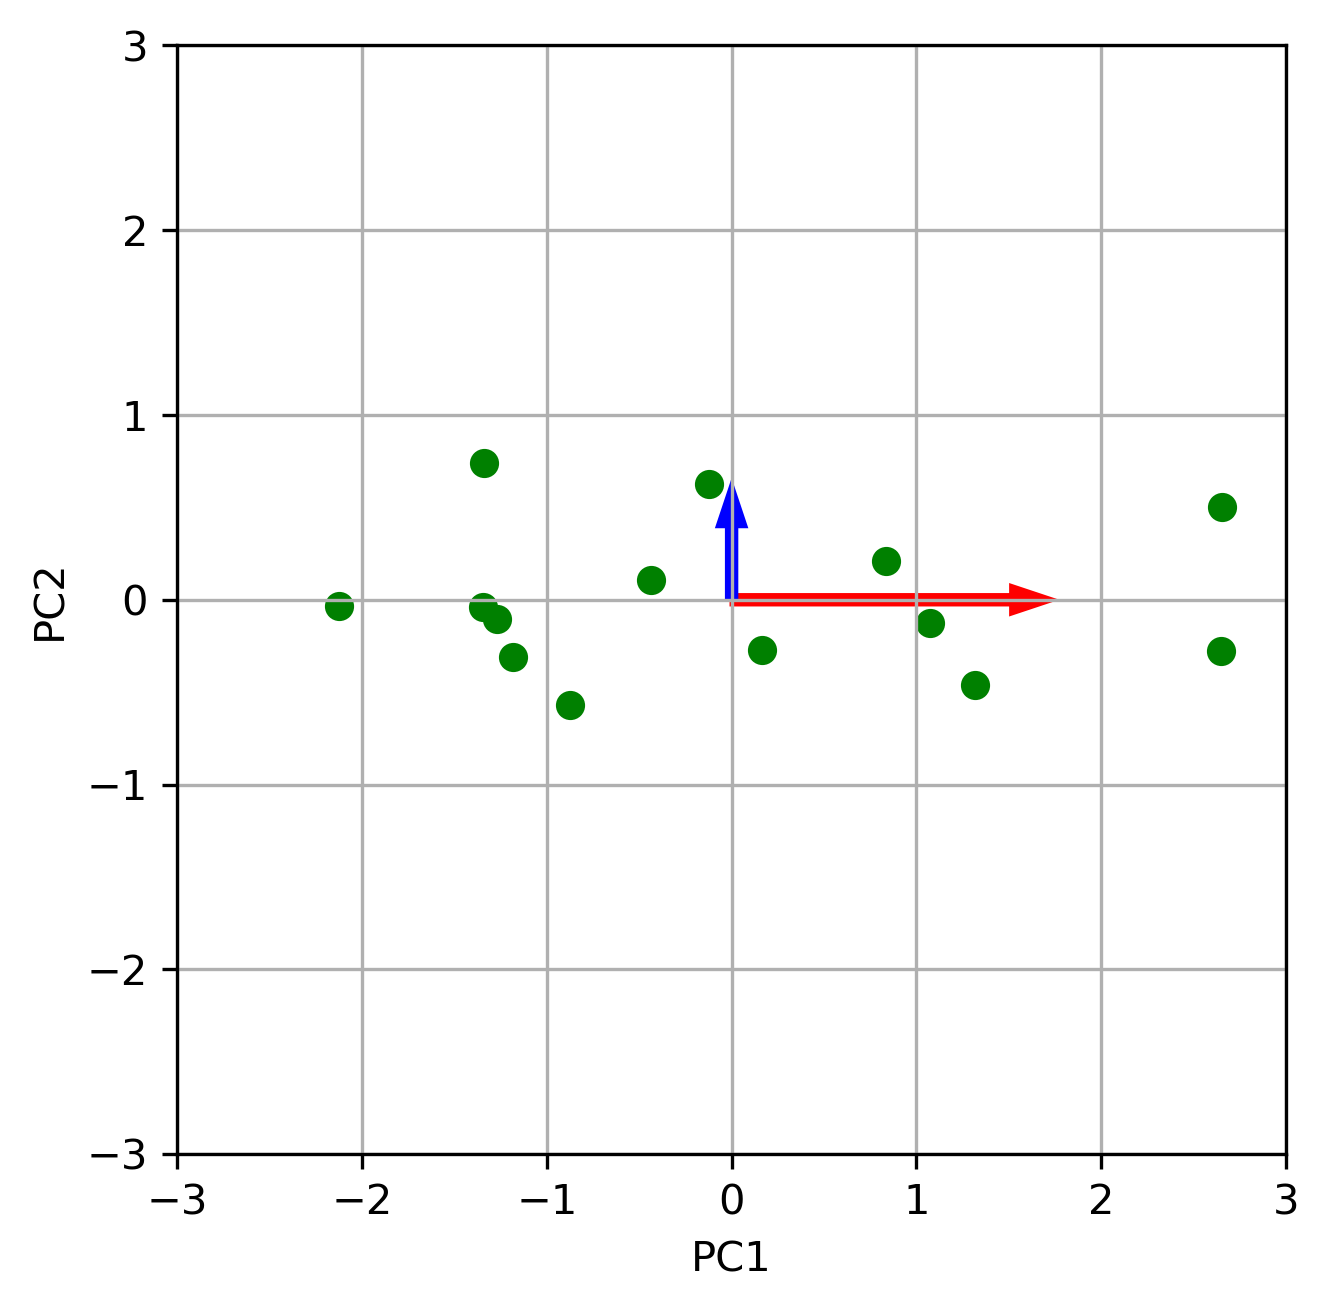
\includegraphics[scale = 0.75]{graphics/PCA_exmp_2.png}\\
The data (green) before and after rotation to the principal axes, with the one with a larger/smaller variance shown as a red/blue arrow.
\end{center}
\begin{center}
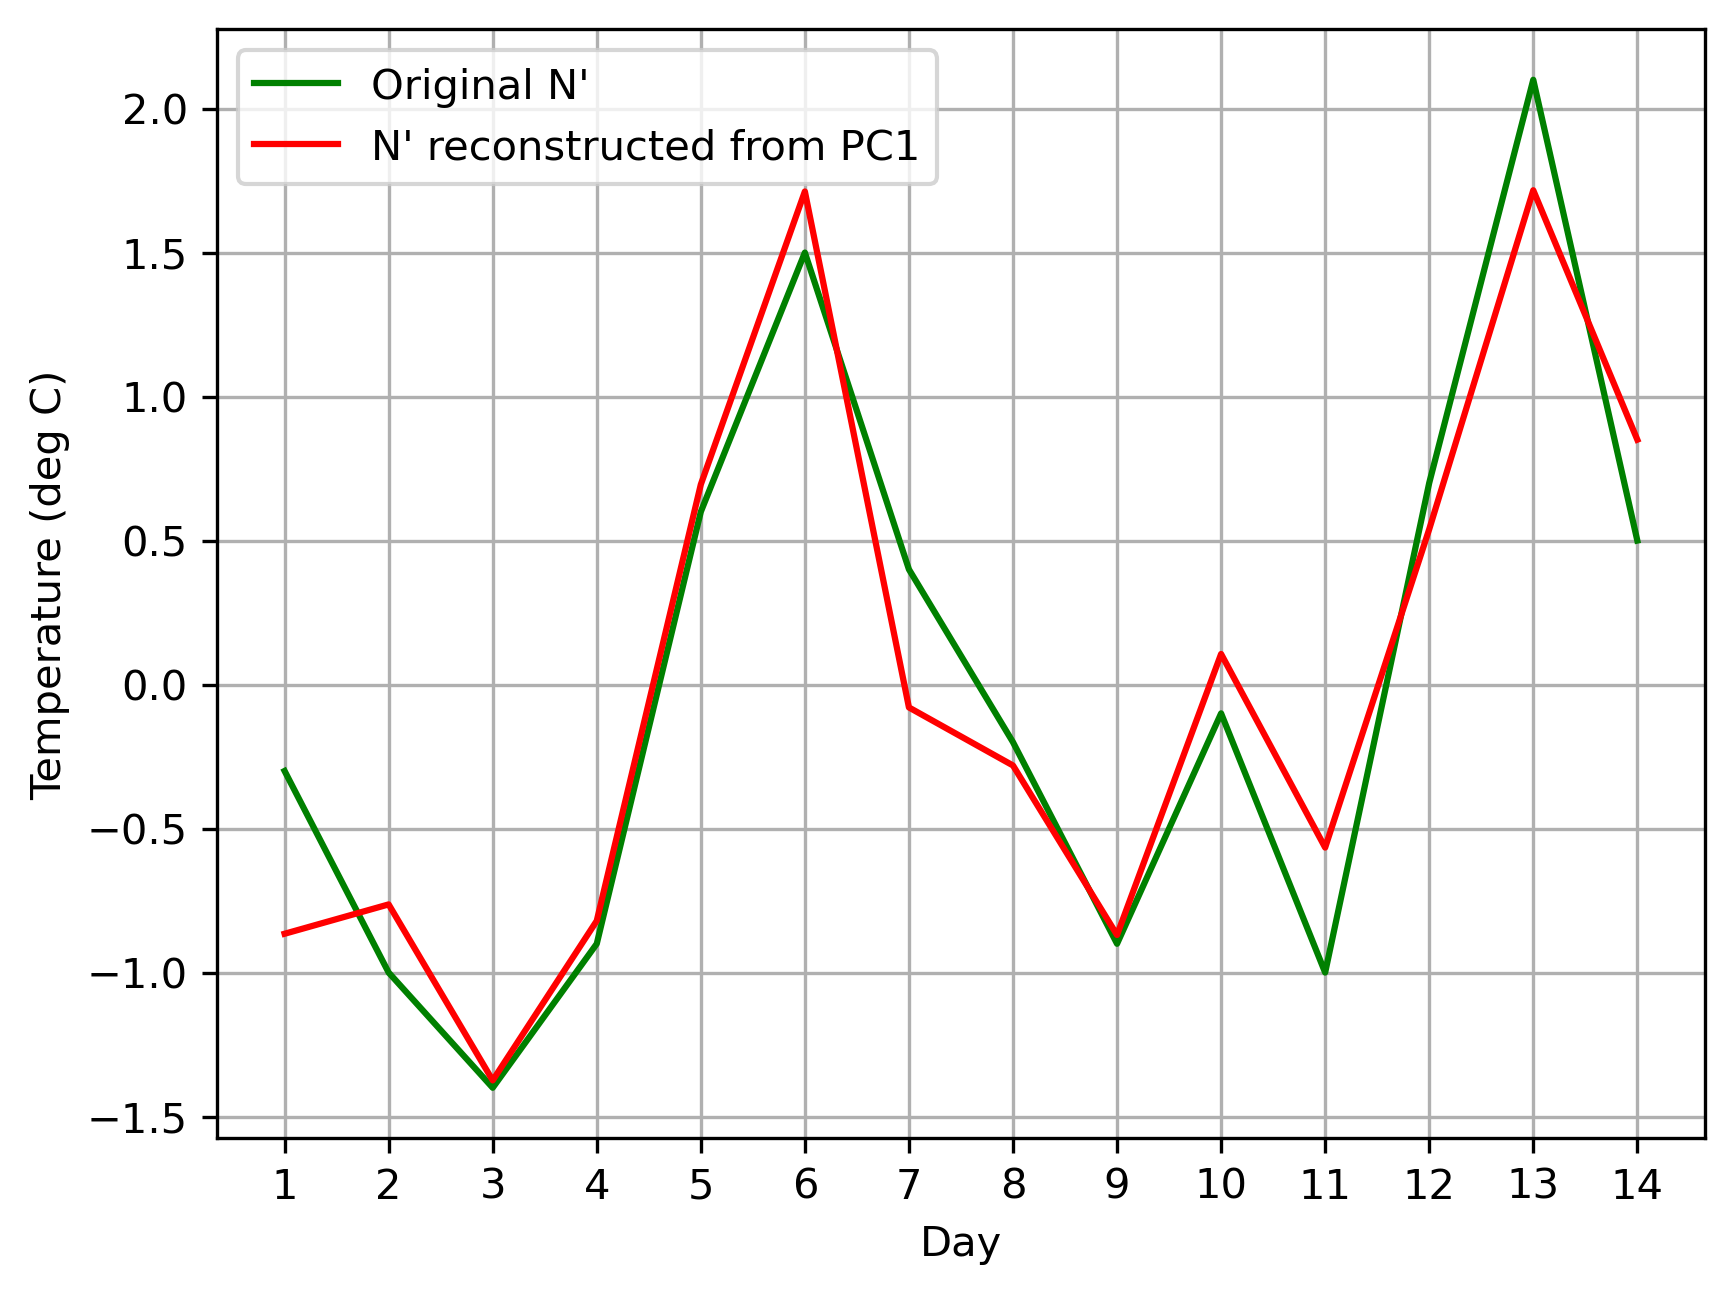
\includegraphics[scale = 0.8]{graphics/PCA_exmp_3.png}\\
Comparison between the original time-series and the one reconstructed using only first PC for $N'$.
\end{center}
\end{solution}

\section{Python Programming}
Since doing EOFs as an Earth Science application is essentially a PCA which has to rely on a computer when the dataset is huge, we will get into the Python programming part first in this chapter. We will need the scikit-learn package (\texttt{sklearn}) for this, and let's use Example \ref{exmp:tempPCA} for demonstration.
\begin{lstlisting}
import numpy as np
from sklearn.decomposition import PCA    

X = np.array([[21.0, 22.3],
              [21.8, 21.6],
              [20.9, 21.2],
              [21.6, 21.7],
              [23.4, 23.2],
              [24.7, 24.1],
              [22.0, 23.0],
              [22.1, 22.4],
              [21.5, 21.7],
              [22.8, 22.5],
              [22.2, 21.6],
              [23.0, 23.3],
              [24.2, 24.7],
              [23.8, 23.1]])
\end{lstlisting}
We have to prepare the data where each column represents the time-series of one variable so the shape of \verb|X| is $(\text{Number of samples}, \text{Number of features})$. Now define a \verb|PCA| object and fit it with the data. We can choose how many PCs to be used, and for now we will keep all of them so that \verb|n_components| $=2$.
\begin{lstlisting}
pca = PCA(n_components=2)
pca.fit(X)    
\end{lstlisting}
We can retrieve the principal directions and variances by
\begin{lstlisting}
print(pca.components_)
print(pca.explained_variance_)    
\end{lstlisting}
which gives
\begin{lstlisting}
[[ 0.76286648  0.64655605]
 [-0.64655605  0.76286648]]
[2.28902525 0.15866706] 
\end{lstlisting}
Notice that the principal directions are arranged in rows so that to get the first one we write \verb|pca.components_[0,:]| that returns \verb|[0.763 0.647]|. The percentage of explained variances are simply computed by
\begin{lstlisting}
print(pca.explained_variance_/np.sum(pca.explained_variance_))
\end{lstlisting}
that returns \verb|[0.9352 0.0648]|. To obtain the time-series of transformed PCs, we simply use the \verb|transform| method:
\begin{lstlisting}
Z = pca.transform(X)
print(Z)
\end{lstlisting}
yielding the expected output of
\begin{lstlisting}
[[-1.33826654  0.74097414]
 [-1.18056259 -0.31027725]
 [-2.12576485 -0.03352339]
 ...
 [ 1.31500445 -0.45908963]]    
\end{lstlisting}
To reconstruct the time-series using only some (the first) PC, we can do the followings.
\begin{lstlisting}
Z_trimmed = np.copy(Z)
Z_trimmed[:,1:] = 0
X_inv = pca.inverse_transform(Z_trimmed)
print(X_inv)
\end{lstlisting}
These generate
\begin{lstlisting}
[[21.47908131 21.73473567]
 [21.59938837 21.83670011]
 [20.87832525 21.22557387]
 ...
 [23.50317282 23.45022409]]    
\end{lstlisting}
equivalent to the last table in Example \ref{exmp:tempPCA} but with the original means included. The following code segments produce the main part of the three plots shown in the example.
\begin{lstlisting}
Y = X - np.mean(X, axis=0)
lambda_1 = pca.explained_variance_[0]
lambda_2 = pca.explained_variance_[1]

plt.scatter(Y[:,0], Y[:,1], color="g")
plt.xlim([-3,3])
plt.ylim([-3,3])
plt.arrow(0,0,lambda_1**0.5*pca.components_[0,0],lambda_1**0.5*pca.components_[0,1], color="r", width=0.05)
plt.arrow(0,0,lambda_2**0.5*pca.components_[1,0],lambda_2**0.5*pca.components_[1,1], color="b", width=0.05)
plt.grid()
plt.gca().set_aspect("equal")
plt.show()

plt.scatter(Z[:,0], Z[:,1], color="g")
plt.xlim([-3,3])
plt.ylim([-3,3])
plt.xlabel("PC1")
plt.ylabel("PC2")
plt.grid()
plt.gca().set_aspect("equal")
plt.show()

plt.plot(np.arange(1,14+1), Y[:,1], color="g", label="Original N'")
plt.plot(np.arange(1,14+1), X_inv[:,1] - np.mean(X, axis=0)[1], color="r", label="N' reconstructed from PC1")
plt.legend()
plt.xticks(np.arange(1,14+1))
plt.show()
\end{lstlisting}

\section{Earth Science Applications: Empirical Orthogonal Functions (EOFs)}
\label{section:EOF}

Here we will read the ERA5 dataset for sea surface temperature (SST) and find the dominant patterns of global SST variability. The data can be retrieved from \href{https://cds.climate.copernicus.eu/datasets/reanalysis-era5-single-levels?tab=download}{https://cds.climate.copernicus.eu/datasets/reanalysis-era5-single-levels?tab=download} and selecting the options "Type: Reanalysis, Variable: Sea surface temperature, Time: 00:00, Data format: NetCDF4". We will choose the time period from 1991 to 2020, every month/day, and a spatial domain from \SI{45}{\degree N} to \SI{45}{\degree S} and \SI{110}{\degree E} to \SI{80}{\degree W}. We will also need the land-sea mask that can be downloaded via \href{https://confluence.ecmwf.int/download/attachments/140385202/lsm_1279l4_0.1x0.1.grb_v4_unpack.nc?version=1&modificationDate=1591983422208&api=v2}{https://confluence.ecmwf.int/download/attachments/\\140385202/lsm\_1279l4\_0.1x0.1.grb\_v4\_unpack.nc?version=1\&modificationDate\\=1591983422208\&api=v2}. Now, import the required packages.
\begin{lstlisting}
import matplotlib.pyplot as plt
import numpy as np
import pandas as pd
import xarray as xr
from sklearn.decomposition import PCA
import cartopy.crs as ccrs
\end{lstlisting}
Load the SST data, work on coarse grids with a $\SI{2.5}{\degree} \times \SI{2.5}{\degree}$ spatial resolution (optional to the reduce computational cost), and exclude leap days.
\begin{lstlisting}
SST_nc = xr.open_dataset("ERA5_SST.nc")
coarse_lat = np.array(SST_nc["latitude"][::10]) # 0.25 deg * 10 = 2.5 deg
coarse_lon = np.array(SST_nc["longitude"][::10])
time = pd.Series(SST_nc["valid_time"])
no_leapdays = ~((time.dt.month == 2) & (time.dt.day == 29))
\end{lstlisting}
Also, prepare the land-sea mask to exclude land grid points and flatten it for indexing later.
\begin{lstlisting}
land_sea_mask_nc = xr.open_dataset("lsm_1279l4_0.1x0.1.grb_v4_unpack.nc")
land_sea_mask = np.array(land_sea_mask_nc["lsm"].sel({"latitude": coarse_lat, "longitude": coarse_lon}, method="nearest")[0, ...])
land_sea_mask = np.where(land_sea_mask > 0, 1, 0)
land_sea_mask_flatten = land_sea_mask.flatten().astype(bool)
\end{lstlisting}
Preprocessing the SST data by subtracting the yearly climatology to acquire the anomaly fields, scale them by the square roots of cosines of the latitudes to account for area weighting and keep only the valid overwater grid points using the land-sea mask:
\begin{lstlisting}
SST_data_arr = np.array(SST_nc["sst"].sel({"latitude": coarse_lat, "longitude": coarse_lon}))
SST_data_arr_no_leap = SST_data_arr[no_leapdays, ...].reshape(30,365,len(coarse_lat),len(coarse_lon))
SST_clim = np.mean(SST_data_arr_no_leap, axis=0)
SST_anomaly = SST_data_arr_no_leap - SST_clim

cos_factor_root = np.cos(np.deg2rad(coarse_lat))**0.5
SST_anomaly_weighted = SST_anomaly * cos_factor_root[None,None,:,None]

SST_flatten = SST_anomaly_weighted.reshape(30*365, len(coarse_lat)*len(coarse_lon))
SST_valid = SST_flatten[:, ~land_sea_mask_flatten]
\end{lstlisting}
Call the PCA and fit it with the prepared, flattened SST data:
\begin{lstlisting}
SST_PCA = PCA(n_components=3) # any number will be fine
SST_PCA.fit(SST_valid)
\end{lstlisting}
Then, recover the latitude-longitude structure of the first PC:
\begin{lstlisting}
PC1 = np.full(len(coarse_lat)*len(coarse_lon), np.nan)
PC1[~land_sea_mask_flatten] = SST_PCA.components_[0,:] # Fill PC1 at appropriate overwater entries
PC1_2D = PC1.reshape(len(coarse_lat), len(coarse_lon)) / cos_factor_root[:,None] # Inverse the cosine factor
\end{lstlisting}
and plot it on the map.
\begin{lstlisting}
plt.figure()
plt.subplot(111, projection=ccrs.PlateCarree(central_longitude=180)) # the central_longitude option is needed to plot across the International Date Line
plt.pcolormesh(coarse_lon, coarse_lat, PC1_2D, cmap="coolwarm", vmin=-0.08, vmax=0.08, transform=ccrs.PlateCarree())
plt.gca().coastlines()
gl = plt.gca().gridlines(draw_labels=True)
gl.top_labels = False
plt.title("First EOF of Sea Surface Temperature (SST) - ENSO")
plt.colorbar(orientation="horizontal", label="Temperature Anomaly (deg C)")
plt.savefig("SST_EOF")
\end{lstlisting}
You should be able to get the following figure.
\begin{center}
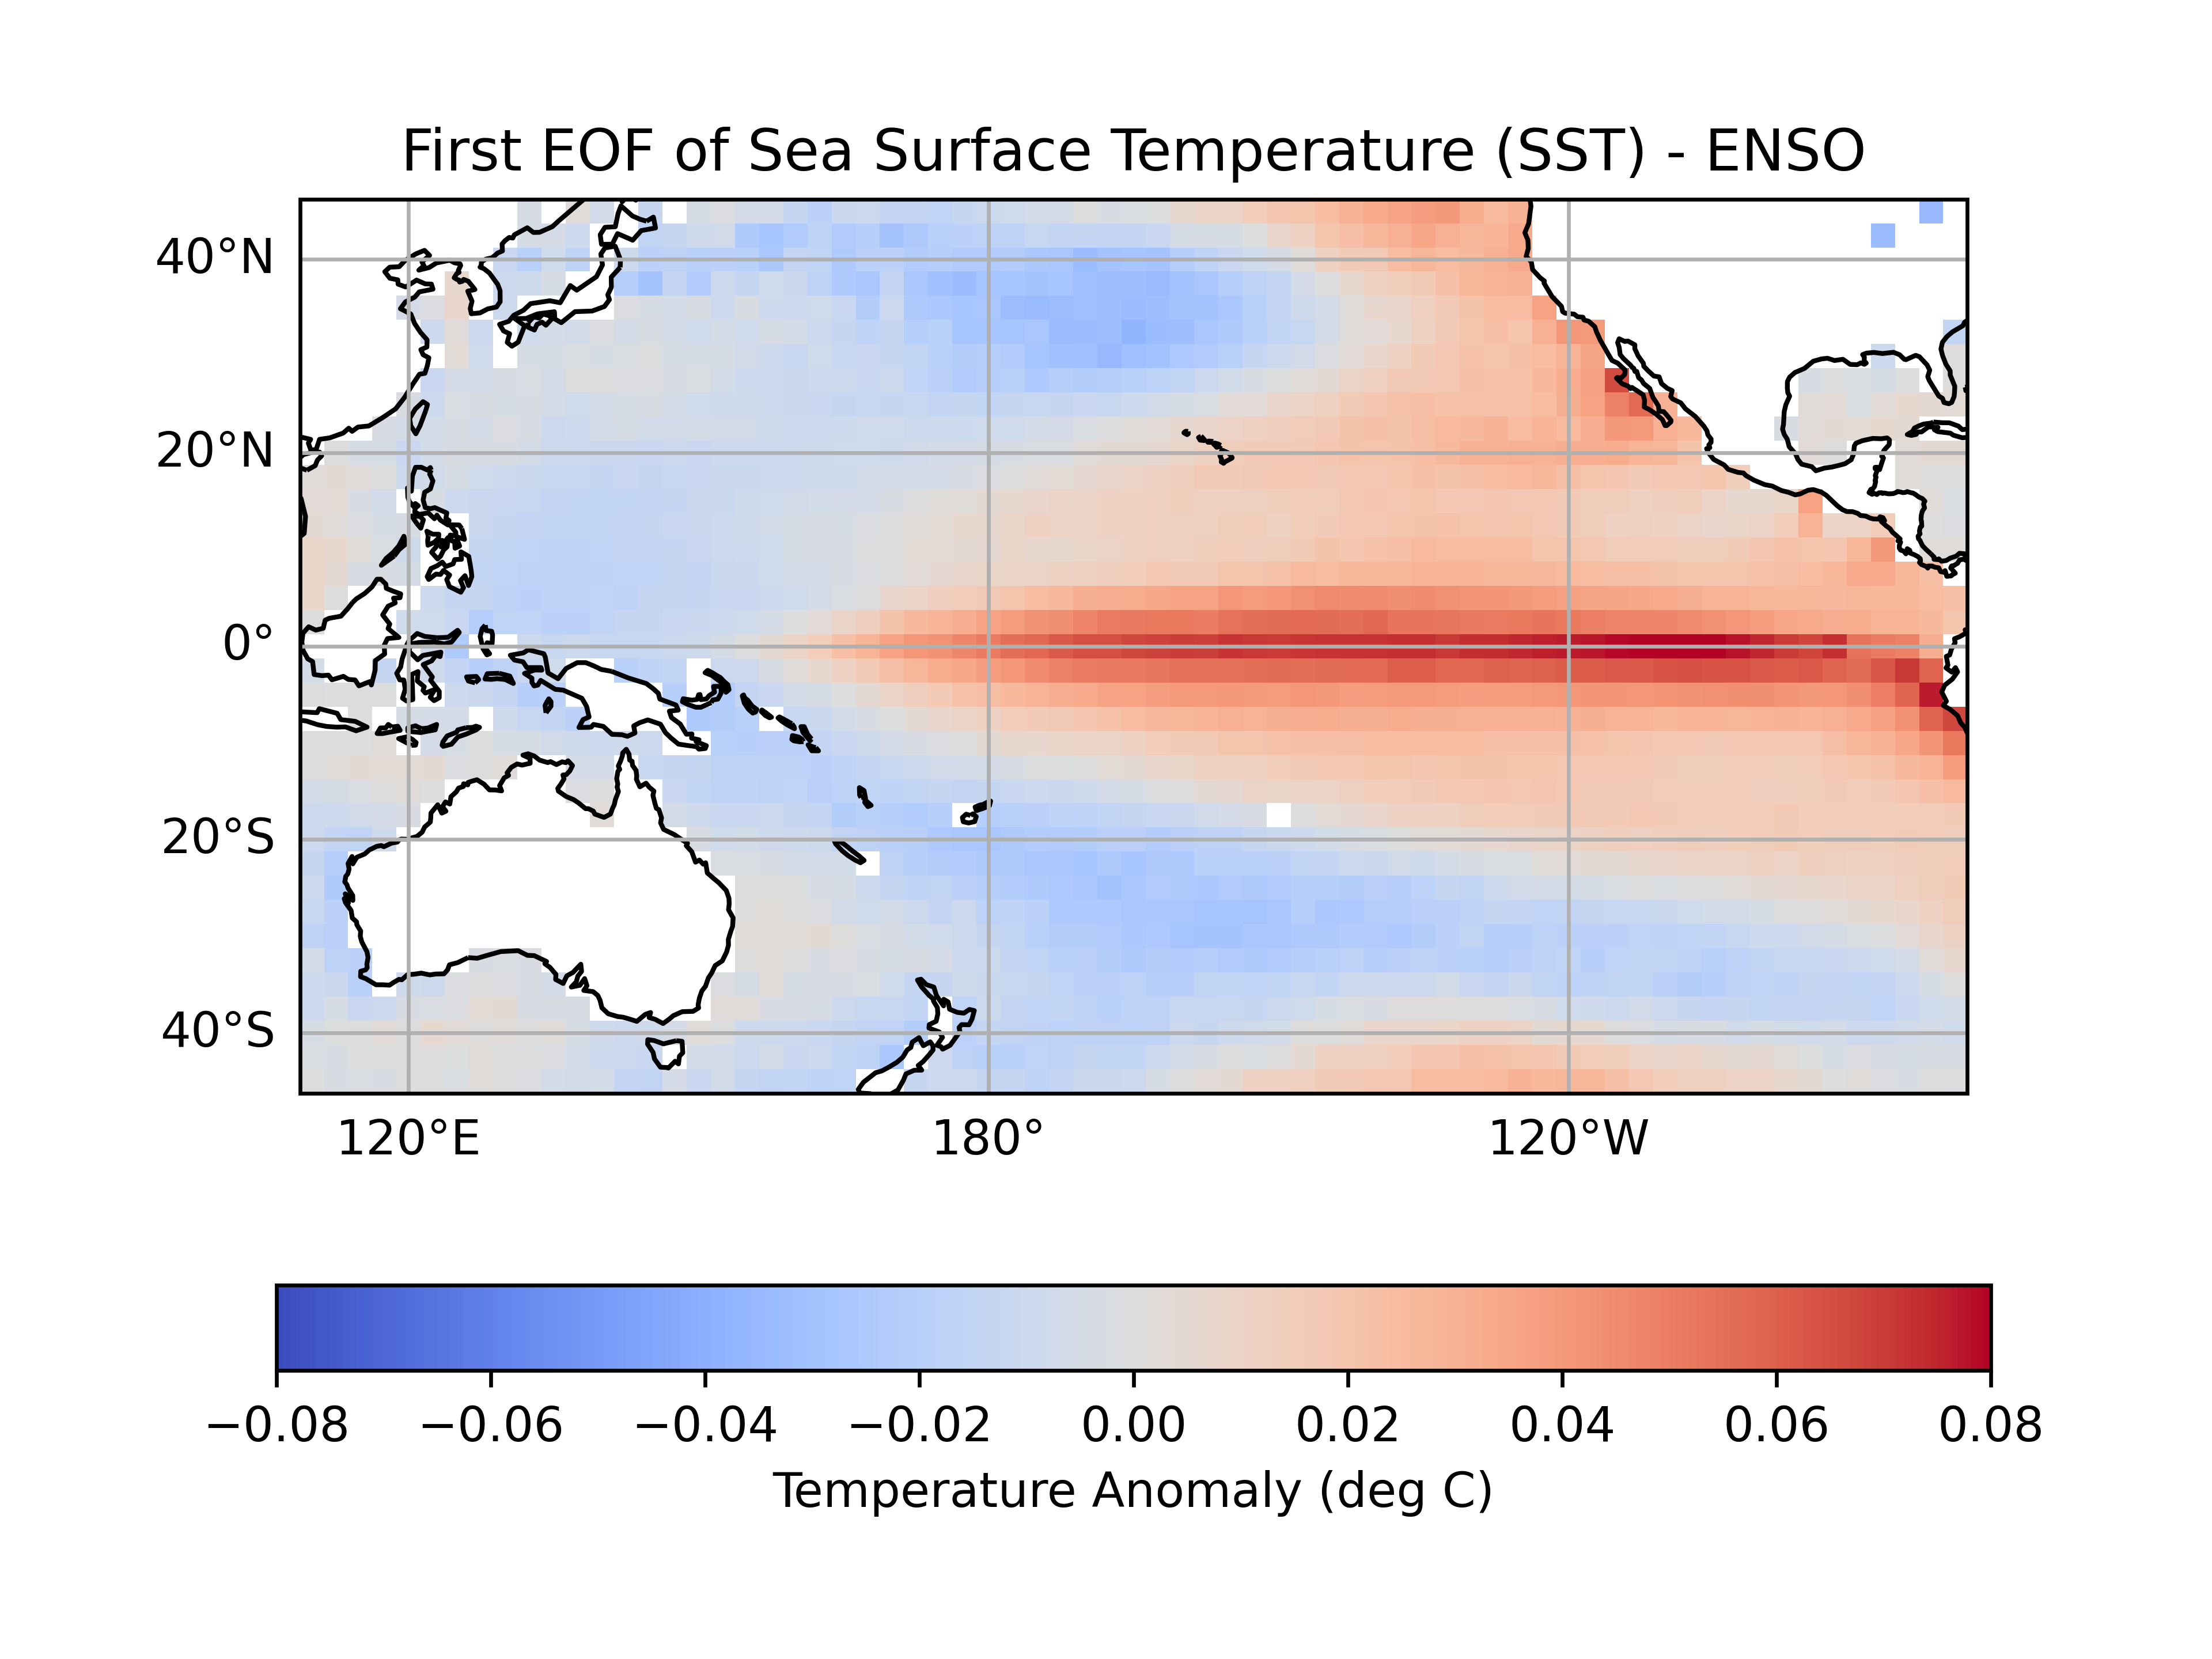
\includegraphics[scale=0.75]{graphics/SST_EOF.png}
\end{center}
This EOF pattern represents the \index{El Niño–Southern Oscillation (ENSO)}\keywordhl{El Niño–Southern Oscillation (ENSO)} phenomenon where the western Pacific gets cooler (warmer) and eastern Pacific becomes warmer (cooler) during the El Niño (La Niña) phase.

\section{Exercise}

\begin{Exercise}
Identify the following conic sections and eliminate the cross-product terms by an appropriate rotation.
\begin{enumerate}[label=(\alph*)]
\item $x^2 + 5xy + 3y^2 = 1$,
\item $x^2 - xy + 2y^2 = 4$,
\item $x^2 + 2xy + y^2 = 1$, what is the graph generated? 
\end{enumerate}
\end{Exercise}

\begin{Exercise}
Find a new expression for the standard hyperbola $y^2 - x^2 = 1$ if a anti-clockwise rotation of $75$ degrees is done. What about a reflection along the $x$-axis?
\end{Exercise}

\begin{Exercise}
Three-dimensional quadrics can also be treated in a similar fashion to two-dimensional conic sections. Find the length of three axes for an ellipsoid $x^2 + y^2 + z^2 + 0.5xy - yz + 0.5xz = 1$ by doing an orthogonal coordinate transformation. What is the requirement for a three-dimensional quadratic form to represent an ellipsoid?
\end{Exercise}

\begin{Exercise}
Use the Sylvester's Law of Inertia to argue that a symmetric matrix $B$ is positive-definite if and only if $B = P^TP$ for some invertible matrix $P$. Hint: Consider $P^T IP$.
\end{Exercise}

\begin{Exercise}
Find the covariance matrix for three pressure time-series over $10$ days at cities $X$, $Y$, $Z$ (in hPa, relative to $1000$ hPa), which take the values
\begin{center}
\begin{tabular}{|c|c|c|}
\hline
$X$ & $Y$ & $Z$ \\
\hline
17.1 & 19.2 & 22.0 \\
\hline
18.5 & 16.9 & 25.4 \\
\hline
14.8 & 15.3 & 17.3 \\
\hline
19.7 & 21.6 & 23.5 \\
\hline
24.1 & 22.3 & 26.8 \\
\hline
21.6 & 20.9 & 23.2 \\
\hline 
28.0 & 26.7 & 29.5 \\
\hline
24.3 & 25.0 & 22.5 \\
\hline
20.3 & 21.5 & 27.2 \\
\hline
23.4 & 22.4 & 24.6 \\
\hline
\end{tabular}
\end{center}
Find the variance of $W = X - 0.5Y - 0.5Z$.
\end{Exercise}

\begin{Exercise}
Carry out Principal Component Analysis on the data set above. Find the Principal Directions and the ratio of explained variance for each of them. Reconstruct the data using the first principal component with largest variance only.
\end{Exercise}

\begin{Exercise}
Download the ERA5 datasets for \SI{200}{hPa} and \SI{850}{hPa} zonal winds, as well as total column water over some $10$ to $20$ years from \SI{15}{\degree N} to \SI{15}{\degree S} and \SI{60}{\degree E} to \SI{160}{\degree E}. Standardize the three variables via dividing them by their standard deviations respectively and follow the procedure outlined in Section \ref{section:EOF} to do the so-called \textit{combined EOFs}. Recover the physical patterns through multiplying the entries of EOF modes by the standard deviations of corresponding variables. You should be able to observe the appearance of \textit{Madden-Julian Oscillation (MJO)} from the first two EOFs. 
\end{Exercise}

